%!TEX root = ../../main.tex
% ============================================================
% 数学\几何作图\三年级.tex
% 本文件由 main.tex 通过 \input 引入，请勿单独编译
% ============================================================


\section{解答：三角形的分割与等腰三角形证明}

\vspace{0.4cm}

\noindent\textbf{1. 把下面的三角形分成两个三角形，并且分出的两个三角形中有一个是等边三角形。}

\vspace{0.6cm}

\begin{center}
\begin{tikzpicture}[>=Stealth, scale=1.3] % 整体思路：先画一个 30°-60°-90° 直角三角形，再取斜边中点，连接到直角顶点，把原图分成一个等边三角形和另一个三角形，并补上角标
  % 顶点坐标：左下角为直角，右下角为30度，计算高度为3，则底边长为3*sqrt(3) ≈ 5.196
  \coordinate (B) at (0, 0);       % 定义左下直角顶点 B
  \coordinate (C) at (5.196, 0);   % 定义右下顶点 C，保证 ∠C=30° 的比例关系
  \coordinate (A) at (0, 3);       % 定义左上顶点 A，保证 ∠A=60°
  
  % 画原三角形的边
  \draw[line width=1.0pt] (A) -- (B) -- (C) -- cycle; % 连接三点并闭合，画出原三角形 ABC
  
  % 直角标记
  \draw[line width=0.8pt] (0.25, 0) -- (0.25, 0.25) -- (0, 0.25); % 在 B 点附近画小方角，表示直角
  
  % 原 30 度角的标记 (在C点)
  \draw[line width=0.8pt] (4.5, 0) arc (180:150:0.7); % 在 C 点附近画角弧，表示 30° 角
  \node[font=\small] at (4.2, 0.2) {$30^\circ$}; % 在角弧附近写出 30°

  % ---------------- 答案作图部分 ----------------
  % 取斜边 AC 的中点 D
  \coordinate (D) at ($(A)!0.5!(C)$); % 取 AC 的中点 D；!0.5! 表示正中点
  
  % 画出分割线 BD
  \draw[red!70!black, line width=1.5pt] (B) -- (D); % 连接 B 与 D，画出分割线 BD
  
  % 为了说明清楚，标注辅助点和角度
  \node[above left] at (A) {$A$}; % 标注点 A
  \node[below left] at (B) {$B$}; % 标注点 B
  \node[below right] at (C) {$C$}; % 标注点 C
  \node[above right] at (D) {$D$}; % 标注点 D

  % 标出等边三角形的角
  \draw[red!70!black, line width=0.8pt] (0, 2.5) arc (-90:-30:0.5); % 在 A 点附近画红色角弧，标出等边三角形中的 60°
  \node[red!70!black, font=\footnotesize] at (0.35, 2.35) {$60^\circ$}; % 写出该角的度数 60°
  
  \draw[red!70!black, line width=0.8pt] (0, 0.5) arc (90:30:0.5); % 在 B 点附近画第二个红色角弧
  \node[red!70!black, font=\footnotesize] at (0.39, 0.65) {$60^\circ$}; % 标出这里也是 60°

  % 角ADB (角2) 的弧线标注 (向左上一点)
  \pic [draw, red!70!black, line width=0.8pt, angle radius=0.6cm] {angle = A--D--B}; % 在 D 点画 ∠ADB 的角弧；angle radius=0.6cm 控制弧半径更大些
  \node[red!70!black, font=\footnotesize] at (1.9, 1.5) {$2$}; % 在该角附近标“角2”

  % 标出另一个三角形的角度
  \draw[red!70!black, line width=0.8pt] (0.7, 0) arc (0:30:0.7); % 在 B 点右侧画另一个角弧，表示分割后另一角
  \node[red!70!black, font=\footnotesize] at (0.9, 0.25) {$1$}; % 在角弧旁标“角1”
  
\end{tikzpicture}
\end{center}

\vspace{0.4cm}

{\small\color{gray}
\textbf{作图说明：} 取斜边 $AC$ 的中点 $D$，连接 $BD$。因为在直角三角形 $ABC$ 中，斜边上的中线等于斜边的一半（$BD = AD$），又因为 $\angle A = 60^\circ$，所以 $\triangle ABD$ 是一个等边三角形。
}

\vspace{0.8cm}

\noindent\textbf{2. 分出的另一个三角形是等腰三角形吗？说明理由。}

\vspace{0.4cm}

\noindent
\textbf{答：}是等腰三角形。

\vspace{0.4cm}

\noindent
\textbf{理由：}\\
如图所示，设原三角形为 $\triangle ABC$，新切分点为 $D$。\\
因为在 $\triangle ABC$ 中，$\angle ABC = 90^\circ$，$\angle C = 30^\circ$，\\
所以 $\angle A = 180^\circ - 90^\circ - 30^\circ = 60^\circ$。\\
既然分出的 $\triangle ABD$ 已经确定是等边三角形，那么 $\angle ABD = 60^\circ$（且左上方的 $\angle 2 = 60^\circ$）。\\
在分出的另一个三角形 $\triangle BDC$ 中：\\
$\angle 1 = \angle ABC - \angle ABD = 90^\circ - 60^\circ = 30^\circ$。\\
因为 $\angle 1 = 30^\circ$ 且 $\angle C = 30^\circ$，即 $\angle 1 = \angle C$，\\
根据“等角对等边”定理可知 $DB = DC$，所以 $\triangle BDC$ 是\textbf{等腰三角形}。

\vspace{0.6cm}

{\small\color{blue!70!black}
\textbf{绘图基本原理与步骤：}\\
\textbf{1. 30-60-90 三角形精确构造}：利用特殊直角三角形比例关系 $1:\sqrt{3}:2$，设竖直边为 3，则水平底边为 $3\sqrt{3} \approx 5.196$。坐标定位 $B(0,0)$、$C(5.196,0)$、$A(0,3)$ 精确还原角度比。\\
\textbf{2. 中点分割}：通过 \texttt{calc} 库的插值算子 \texttt{(A)!0.5!(C)} 自动取斜边 $AC$ 的中点 $D$，连接 $BD$ 即为答案分割线（红色 \texttt{red!70!black} 加粗区分答案图层）。\\
\textbf{3. 角度标注}：使用 \texttt{arc} 命令绘制 $30^\circ$、$60^\circ$ 角弧，并用 \texttt{pic[angle]} 指令渲染角 $\angle ADB$ 的弧线标记。红色统一用于答案绘制图层，与黑色原图形成主次分层。
}



\section{解答：在图中涂色表示分数}

\vspace{0.4cm}

\noindent\textbf{1. 在图中涂色表示它下面的分数。}

\vspace{0.8cm}

\begin{center}
\begin{tikzpicture}[>=Stealth, scale=0.85, line width=1pt] % 整体思路：三幅图分别通过“平均分后涂色”的方式表示分数，因此每一幅都先画外形或网格，再填充对应份数，最后在下方标分数

  % 1. 正方形网格 3x3
  \begin{scope}[shift={(0,0)}] % 第一幅图保持在左侧原位
    \fill[black!70] (0, 2) rectangle (3, 3); % 先把最上面一整行 3 个小正方形涂黑；rectangle 表示用对角点画矩形
    \fill[black!70] (0, 1) rectangle (2, 2); % 再把中间一行左边 2 个小格涂黑，这样一共涂了 5 个小格
    \draw[line width=0.8pt, step=1cm] (0,0) grid (3,3); % 画 3×3 网格；step=1cm 表示每一格边长 1cm；line width=0.8pt 为细边框
    \node[below=15pt, font=\Large] at (1.5, 0) {$\frac{5}{9}$}; % 在图下方 15pt 处写出分数 5/9
  \end{scope} % 结束第一幅正方形网格图

  % 2. 平行四边形
  \begin{scope}[shift={(5.5,0)}] % 第二幅图整体右移 5.5cm
    % 涂色区域 (左上角子平行四边形)
    \fill[black!70] (0.75, 1.5) -- (1.95, 1.5) -- (2.7, 3) -- (1.5, 3) -- cycle; % 用四个顶点围成一个小平行四边形并填黑，表示 4 份中的 1 份；cycle 自动闭合图形
    % 外框
    \draw[line width=0.8pt] (0,0) -- (2.4,0) -- (3.9,3) -- (1.5,3) -- cycle; % 画大平行四边形外框
    % 分割线
    \draw[line width=0.8pt] (1.2,0) -- (2.7,3); % 画一条与侧边平行的分割线，把图形纵向分成两份
    \draw[line width=0.8pt] (0.75,1.5) -- (3.15,1.5); % 再画一条水平样式的分割线，把图形横向分成两份，最终得到 4 等份
    % 分数
    \node[below=15pt, font=\Large] at (1.95, 0) {$\frac{1}{4}$}; % 在图下方标出对应分数 1/4
  \end{scope} % 结束第二幅平行四边形分数图

  % 3. 椭圆与圆圈
  \begin{scope}[shift={(13.5, 1.5)}] % 第三幅图右移并略上移，让椭圆与前两图对齐
    % 椭圆外框
    \draw[line width=0.8pt] (0, 0) ellipse (3.6cm and 1.6cm); % 以原点为中心画椭圆；横半轴 3.6cm，纵半轴 1.6cm，表示整体“1”的容器
    
    % 排列圆圈 (2行 x 5列)
    \foreach \x in {-2, -1, 0, 1, 2} { % 外层循环控制 5 列圆圈的位置
      \foreach \y in {-0.6, 0.6} { % 内层循环控制上下两行圆圈的位置
        \ifnum \x<1 % 条件判断：当前列编号若小于 1，就属于左边 3 列，需要涂黑
          % 涂黑的圆圈 (左边 3 列共 6 个)
          \filldraw[fill=black!85, draw=black, line width=0.8pt] (\x*1.1, \y) circle (0.35cm); % filldraw 同时画轮廓并填充；圆心坐标由 \x*1.1 和 \y 给出；circle (0.35cm) 表示半径 0.35cm
        \else
          % 空白圆圈 (右边 2 列共 4 个)
          \draw[line width=0.8pt] (\x*1.1, \y) circle (0.35cm); % 对右边两列只画空心圆，不填色
        \fi
      }
    }
    % 分数
    \node[below=15pt, font=\Large] at (0, -1.5) {$\frac{3}{5}$}; % 在椭圆下方写出分数 3/5
  \end{scope} % 结束第三幅“圆圈分组”分数图

\end{tikzpicture}
\end{center}

\vspace{0.6cm}
{\small\color{gray}
\textbf{解析：}\\
1. $\frac{5}{9}$：把正方形平均分成 $9$ 份，涂色部分占其中的 $5$ 份（涂满上方的 $3$ 个和中间行左侧的 $2$ 个小正方形）。\\
2. $\frac{1}{4}$：把平行四边形平均分成 $4$ 份，涂色部分占其中的 $1$ 份（本题涂满左上方的 $1$ 个平行四边形）。\\
3. $\frac{3}{5}$：共有 $10$ 个圆圈，平均分作 $5$ 份，每份 $2$ 个。$\frac{3}{5}$ 表示取其中的 $3$ 份，即 $2 \times 3 = 6$ 个圆圈，故将左侧的 $6$ 个小圆圈全部涂成黑色实体。
}

\vspace{0.8cm}


\vspace{0.6cm}

{\small\color{blue!70!black}
\textbf{绘图基本原理与步骤：}\\
\textbf{1. 坐标定位与几何构建}：根据题意中的已知长度和角度，使用 \texttt{coordinate} 定义关键顶点坐标，通过 \texttt{draw} 指令按序连接成完整几何图形。线宽、颜色参数区分原图（黑色）与答案（红色 \texttt{red!70!black}）图层。\\
\textbf{2. 辅助量标注}：利用 \texttt{node} 的方向锚点（\texttt{above}、\texttt{below}、\texttt{left}、\texttt{right}）将角度、边长、面积等数据标注在图形周围，避免与线条或其他标注重叠。若涉及角弧则使用 \texttt{arc} 或 \texttt{pic[angle]} 命令渲染。\\
\textbf{3. 虚实线分层}：题干已知条件用实线绘制，解答新增的辅助线或操作痕迹用 \texttt{dashed} 虚线或彩色加粗线标识，确保读者一眼区分原有信息与作答内容。
}

%% ==============================
%% 分数、小数、百分数互化
%% ==============================
\newpage



\section{解答：六边形的分数涂色}

\vspace{0.6cm}

\textbf{\LARGE 82.} \textbf{将每个六边形分别涂色表示下面的分数。\\[1ex]
第一图下标注：$\displaystyle\frac{1}{2}$ \qquad 第二图下标注：$\displaystyle\frac{1}{3}$ \qquad 第三图下标注：$\displaystyle\frac{1}{6}$}

\vspace{0.4cm}
\textbf{解：}

\textbf{分析：}
如图所示，每个正六边形都被内部相交的三条对角线平均分成了 $6$ 个完全相同的小正三角形。
要表示特定的分数，只需要计算应涂色的小三角形数量：
1. 第一图表示 $\displaystyle\frac{1}{2}$：需要涂色总块数的 $\displaystyle\frac{1}{2}$，即 $6 \times \frac{1}{2} = 3$ 块。
2. 第二图表示 $\displaystyle\frac{1}{3}$：需要涂色总块数的 $\displaystyle\frac{1}{3}$，即 $6 \times \frac{1}{3} = 2$ 块。
3. 第三图表示 $\displaystyle\frac{1}{6}$：需要涂色总块数的 $\displaystyle\frac{1}{6}$，即 $6 \times \frac{1}{6} = 1$ 块。

\vspace{0.6cm}
\begin{center}
\begin{tikzpicture}[>=Stealth, scale=1.6]

  % 定义绘制一个被6等分的正六边形的宏
  % 参数1: x位移
  \def\drawHexagon#1{
    \begin{scope}[shift={(#1, 0)}]
      % 画六边形外框
      \draw[line width=1pt] (0:1) \foreach \i in {1,2,3,4,5} { -- (\i*60:1) } -- cycle;
      % 画三条虚线对角线
      \draw[dashed, line width=0.6pt] (0:1) -- (180:1);
      \draw[dashed, line width=0.6pt] (60:1) -- (240:1);
      \draw[dashed, line width=0.6pt] (120:1) -- (300:1);
    \end{scope}
  }

  % 第一个图形：涂 3 块 (1/2)
  \begin{scope}[shift={(0,0)}]
    % 填充 0~180 度的 3 个小正三角形
    \fill[blue!30] (0,0) -- (0:1) \foreach \i in {1,2,3} { -- (\i*60:1) } -- cycle;
    \drawHexagon{0}
    \node[below, font=\Large] at (0, -1.2) {$\displaystyle\frac{1}{2}$};
  \end{scope}

  % 第二个图形：涂 2 块 (1/3)
  \begin{scope}[shift={(3.5,0)}]
    % 填充 60~180 度的 2 个小正三角形 (顶部及左上)
    \fill[blue!30] (0,0) -- (60:1) \foreach \i in {2,3} { -- (\i*60:1) } -- cycle;
    \drawHexagon{0}
    \node[below, font=\Large] at (0, -1.2) {$\displaystyle\frac{1}{3}$};
  \end{scope}

  % 第三个图形：涂 1 块 (1/6)
  \begin{scope}[shift={(7,0)}]
    % 填充 60~120 度的 1 个小正三角形 (正上方)
    \fill[blue!30] (0,0) -- (60:1) -- (120:1) -- cycle;
    \drawHexagon{0}
    \node[below, font=\Large] at (0, -1.2) {$\displaystyle\frac{1}{6}$};
  \end{scope}

\end{tikzpicture}
\end{center}

\vspace{0.4cm}
{\small\color{blue!70!black}
\textbf{绘图原理与步骤：}\\
\textbf{1. 极坐标正多边形生成：} 利用极坐标系循环生成法 \texttt{(A:R)} 快速渲染完全标准正六边形，设定外接圆定长半径为 $1$。并人为规定顶点的极角依次为 $0^\circ, 60^\circ, 120^\circ \dots 300^\circ$。这一设定不仅确保了图形的顶边与底边绝对水平，且使得连接 $0^\circ$ 和 $180^\circ$ 的对角线刚好是一根完美的水平中轴线，与原题素材的物理放置姿态完全锲合。\\
\textbf{2. 均等基本块划分：} 通过追加 \texttt{\textbackslash draw[dashed]} 指令连接全部核心对角线，实现在渲染外框的同时，在图形内部打通了隔断线。物理上将原本致密的整块大正六边形成功均分为 $6$ 块等面积的正三角形阵列单元。\\
\textbf{3. 分割填色法则：} 将题目提出的代数分数逻辑映射为涂色数量逻辑（$1/2\to 3$ 块，$1/3\to 2$ 块，$1/6\to 1$ 块）。然后启用特定的区块填充层 \texttt{\textbackslash fill[blue!30]}，精确约束中心 $(0,0)$ 延伸到外围对应节点之间的扇形发散式多边形面域，彻底杜绝手工填充导致的色彩溢出或留白死角。
}

%% ==============================
%% 第92题（补充题）：用不同方法表示正方形的 1/4
%% ==============================
\newpage



\section{解答：表示分数的多种折叠模型}

\vspace{0.6cm}

\textbf{\LARGE 83.} \textbf{（第 4 题）你能用不同的方法表示每个正方形的 $\displaystyle\frac{1}{4}$ 吗？先用纸折一折，再画一画。}

\vspace{0.4cm}
\textbf{解：}

\textbf{分析：}
要把正方形平均分成 $4$ 份并着色表示出其中的 $\displaystyle\frac{1}{4}$，常见的基于对称性的折法（等分法）共有以下 4 种典型图案：
1. \textbf{竖向等分}：将正方形往同一方向连续对折两次，得到 4 个相同高度的竖直长条。涂色其中 1 块。
2. \textbf{横向等分}：与竖向等分同理，得到 4 个相同宽度的横向长条。涂色其中 1 块。
3. \textbf{十字等分}：横向和纵向各中心对折一次，得到 4 个相同的小正方形。涂色其中 1 块小正方形。
4. \textbf{对角线等分}：沿着正方形的两条对角线分别对折，得到 4 个相同的等腰直角三角形。涂色其中 1 块。

\vspace{0.6cm}
\begin{center}
\begin{tikzpicture}[>=Stealth, x=2.2cm, y=2.2cm]

  % 提取绘制单体正方形的宏
  \def\drawSquare#1{
    % 画实线外框
    \draw[line width=1pt] (#1, 0) rectangle (#1+1, 1);
  }

  % 1. 竖向四等分
  \begin{scope}[shift={(0,0)}]
    % 涂色第一条
    \fill[blue!20] (0, 0) rectangle (0.25, 1);
    \drawSquare{0}
    % 画分划虚线
    \draw[dashed, line width=0.6pt] (0.25, 0) -- (0.25, 1);
    \draw[dashed, line width=0.6pt] (0.5,  0) -- (0.5,  1);
    \draw[dashed, line width=0.6pt] (0.75, 0) -- (0.75, 1);
    \node[below, font=\small] at (0.5, -0.25) {方法一};
  \end{scope}

  % 2. 纵向四等分（横向长条）
  \begin{scope}[shift={(1.4,0)}]
    % 涂色最下一条
    \fill[blue!20] (0, 0) rectangle (1, 0.25);
    \drawSquare{0}
    \draw[dashed, line width=0.6pt] (0, 0.25) -- (1, 0.25);
    \draw[dashed, line width=0.6pt] (0, 0.5)  -- (1, 0.5);
    \draw[dashed, line width=0.6pt] (0, 0.75) -- (1, 0.75);
    \node[below, font=\small] at (0.5, -0.25) {方法二};
  \end{scope}

  % 3. 十字四等分
  \begin{scope}[shift={(2.8,0)}]
    % 涂色左下角小正方形
    \fill[blue!20] (0, 0) rectangle (0.5, 0.5);
    \drawSquare{0}
    \draw[dashed, line width=0.6pt] (0.5, 0) -- (0.5, 1);
    \draw[dashed, line width=0.6pt] (0, 0.5) -- (1, 0.5);
    \node[below, font=\small] at (0.5, -0.25) {方法三};
  \end{scope}

  % 4. 对角线四等分
  \begin{scope}[shift={(4.2,0)}]
    % 涂色下方三角形
    \fill[blue!20] (0, 0) -- (1, 0) -- (0.5, 0.5) -- cycle;
    \drawSquare{0}
    \draw[dashed, line width=0.6pt] (0, 0) -- (1, 1);
    \draw[dashed, line width=0.6pt] (0, 1) -- (1, 0);
    \node[below, font=\small] at (0.5, -0.25) {方法四};
  \end{scope}

\end{tikzpicture}
\end{center}

\vspace{0.4cm}
{\small\color{blue!70!black}
\textbf{绘图原理与步骤：}\\
\textbf{1. 图元定位阵列：} 建立坐标域，定义基础正方形内部比例常数为 $1$。分别于 $x=0, 1.4, 2.8, 4.2$ 的偏移处并行铺设四个基准大实体正方形外框，还原原题干中横向并排依次排开的四大方框环境。\\
\textbf{2. 几何代数等分模型：} 展现物理操作的“折纸”效果即是向框架内追加平分级的辅助线。针对等分这一严密的数学命题，分别编写了三等距绝对垂直律、绝对水平分割律、正交十字对偶中心律以及点对称极限折痕（交叉对角）等四种拓扑方程，通过 \texttt{dashed} 属性赋予拆分折痕。\\
\textbf{3. 独立集块高亮着色：} 利用 \texttt{\textbackslash fill[blue!20]} 的特定区域填充功能，对于矩形切块严格采用 \texttt{rectangle} 参数矩阵锁死，对于三角切块则采用闭环多边形连线 \texttt{cycle} 限位，强行高亮出四种形态截然不同但面积恒等占比 $1/4$ 的比例单元。
}


%% ==============================
%% 第93题（补充题）：分数涂色与大小比较
%% ==============================
\vspace{1.5cm}

\textbf{\LARGE 84.} \textbf{（第 3 题）先涂色表示分数，再比较每组分数的大小。}

\vspace{0.4cm}
\textbf{解：}

\textbf{分析：}
比较给定的两组真分数：
1. 第一组：同分母分数 $\displaystyle\frac{3}{8}$ 与 $\displaystyle\frac{5}{8}$ 比较。分母相同代表切分的标准块大小一样，此时“分子越大，分数实际所占的面积就越大”，故 $\displaystyle\frac{3}{8} < \displaystyle\frac{5}{8}$。
对应在图上的视觉直观操作：每个大正方形已被细分为 $8$ 个等分小三角形，在左图中涂去 $3$ 个，在右图中涂去 $5$ 个，清晰可见右侧涂色区更大。
2. 第二组：同分母分数 $\displaystyle\frac{3}{4}$ 与 $\displaystyle\frac{2}{4}$ 比较。同理，由分子数值可判明 $\displaystyle\frac{3}{4} > \displaystyle\frac{2}{4}$。
在图上的动作：每个大正方形已被切分为 $4$ 个等分小方格，左图按分子占涂 $3$ 个，右图涂 $2$ 个即见大小高低。

\vspace{0.6cm}
\begin{center}
\begin{tikzpicture}[>=Stealth, x=1.8cm, y=1.8cm]

  %% 第一组：3/8 与 5/8
  \begin{scope}[shift={(0,0)}]
    % 左边正方形 (3/8)
    \begin{scope}[shift={(0,0)}]
      % 涂 3 个小三角形
      \fill[blue!30] (0.5, 0.5) -- (0,0) -- (0.5,0) -- cycle;
      \fill[blue!30] (0.5, 0.5) -- (0.5,0) -- (1,0) -- cycle;
      \fill[blue!30] (0.5, 0.5) -- (1,0) -- (1,0.5) -- cycle;
      
      % 外框
      \draw[line width=1pt] (0,0) rectangle (1,1);
      % 米字分割线
      \draw[dashed, line width=0.6pt] (0.5,0) -- (0.5,1);
      \draw[dashed, line width=0.6pt] (0,0.5) -- (1,0.5);
      \draw[dashed, line width=0.6pt] (0,0) -- (1,1);
      \draw[dashed, line width=0.6pt] (0,1) -- (1,0);
    \end{scope}

    % 右边正方形 (5/8)
    \begin{scope}[shift={(1.4,0)}]
      % 涂 5 个小三角形
      \fill[blue!30] (0.5, 0.5) -- (0,0) -- (0.5,0) -- cycle;
      \fill[blue!30] (0.5, 0.5) -- (0.5,0) -- (1,0) -- cycle;
      \fill[blue!30] (0.5, 0.5) -- (1,0) -- (1,0.5) -- cycle;
      \fill[blue!30] (0.5, 0.5) -- (1,0.5) -- (1,1) -- cycle;
      \fill[blue!30] (0.5, 0.5) -- (1,1) -- (0.5,1) -- cycle;
      
      % 外框
      \draw[line width=1pt] (0,0) rectangle (1,1);
      % 米字分割线
      \draw[dashed, line width=0.6pt] (0.5,0) -- (0.5,1);
      \draw[dashed, line width=0.6pt] (0,0.5) -- (1,0.5);
      \draw[dashed, line width=0.6pt] (0,0) -- (1,1);
      \draw[dashed, line width=0.6pt] (0,1) -- (1,0);
    \end{scope}

    % 下方分数及比较圆圈符号
    \node[anchor=mid, font=\Large] at (0.5, -0.6) {$\displaystyle\frac{3}{8}$};
    \draw[line width=0.8pt] (1.2, -0.6) circle (0.2);
    \node[anchor=mid, font=\large] at (1.2, -0.6) {$<$};
    \node[anchor=mid, font=\Large] at (1.9, -0.6) {$\displaystyle\frac{5}{8}$};
  \end{scope}


  %% 第二组：3/4 与 2/4
  \begin{scope}[shift={(4.5,0)}]
    % 左边正方形 (3/4)
    \begin{scope}[shift={(0,0)}]
      % 涂 3 个小正方形
      \fill[blue!30] (0,0) rectangle (1,0.5);
      \fill[blue!30] (0,0.5) rectangle (0.5,1);
      
      % 外框
      \draw[line width=1pt] (0,0) rectangle (1,1);
      % 十字分割线
      \draw[dashed, line width=0.6pt] (0.5,0) -- (0.5,1);
      \draw[dashed, line width=0.6pt] (0,0.5) -- (1,0.5);
    \end{scope}

    % 右边正方形 (2/4)
    \begin{scope}[shift={(1.4,0)}]
      % 涂 2 个小正方形
      \fill[blue!30] (0,0) rectangle (1,0.5);
      
      % 外框
      \draw[line width=1pt] (0,0) rectangle (1,1);
      % 十字分割线
      \draw[dashed, line width=0.6pt] (0.5,0) -- (0.5,1);
      \draw[dashed, line width=0.6pt] (0,0.5) -- (1,0.5);
    \end{scope}

    % 下方分数及比较圆圈符号
    \node[anchor=mid, font=\Large] at (0.5, -0.6) {$\displaystyle\frac{3}{4}$};
    \draw[line width=0.8pt] (1.2, -0.6) circle (0.2);
    \node[anchor=mid, font=\large] at (1.2, -0.6) {$>$};
    \node[anchor=mid, font=\Large] at (1.9, -0.6) {$\displaystyle\frac{2}{4}$};
  \end{scope}

\end{tikzpicture}
\end{center}

\vspace{0.4cm}
{\small\color{blue!70!black}
\textbf{绘图原理与步骤：}\\
\textbf{1. 域隔离对比系：} 利用两个独立包裹的 \texttt{scope} （平移量相隔足够宽距）宏观分区建立了两套绝对独立的对照绘图区。左侧为八等分体系，右侧为基准十字四等分体系，保持所有方块外延尺寸严密一致并排布局，彻底实现原题左右互不干扰的并排比列版面。\\
\textbf{2. 细分网格裁切场：} 对于“涂色表示分数的实质计算”，必须对空白基板做等效切分：左侧区域通过对角线加横竖中位线簇（施加 \texttt{dashed} 点划线属性）切割成 $8$ 个“全边等底正三角”；右侧区域则仅走单纯的十字正中切分分离为 $4$ 个纯正方微块块，为底层的数据结构绑定图元。\\
\textbf{3. 分区面积映射法则：} 紧扣两组代数算子中的分子系数（$3、5$ 及 $3、2$），指令程序采用天蓝色（\texttt{blue!30}）精确检索并吞噬掉对应个数的微型切块。并在最后一行布置底注级渲染——用中心坐标 \texttt{anchor=mid} 精准压平实线评判空圆圈，同时往圆心中注入机器级准确判断的 $<$ 及 $>$ 等比例排版的矢量不等号。
}

%% ==============================
%% 第94题（补充题）：等值分数涂色
%% ==============================
\newpage



\section{解答：等值分数的涂色与转化}

\vspace{0.6cm}

\textbf{\LARGE 85.} \textbf{先在图中涂色表示已知分数的等值分数，再填空。}

\vspace{0.4cm}
\textbf{解：}

\textbf{分析：}
“等值分数”是指虽然分子分母的数字不同，但其表示的实质数值（在一个固定大小的图形中即指代对应相等的覆盖面积）永远相等的分数。
1. 第一个图形组：左侧的六边形被极点射线分成了 $3$ 个并排的菱形，阴影部分占据 $1$ 个菱形，即表示 $\displaystyle\frac{1}{3}$。为了保证面积的绝对“等值”，右侧的六边形（已被全等切分为 $6$ 个小正三角形）其涂色区域必须与左图一致（占据左半边），此时刚好吞并了 $2$ 块小三角形，故得出等价分数公式 $\displaystyle\frac{1}{3} = \frac{2}{6}$。
2. 第二个图形组：左侧的正方形横向等分切成了 $4$ 份水平层，顶层被涂成了灰色，客观表示 $\displaystyle\frac{1}{4}$。而在右侧的正方形中，整个画面被进一步碎化成 $4 \times 4 = 16$ 个同尺寸的小方格，要想使得涂色面积与左边高度吻合一致，那就必须涂满第一排平行的 $4$ 个小方格，由此得出 $\displaystyle\frac{1}{4} = \frac{4}{16}$。

\vspace{0.6cm}
\begin{center}
\begin{tikzpicture}[>=Stealth, line width=0.8pt]

  %% ========== 1. 左侧六边形组 (1/3 和 2/6) ==========
  \begin{scope}[shift={(0,0)}]
    \def\R{1.4}
    % 左一：涂灰色 (题干要求)
    \fill[gray!30] (0,0) -- (120:\R) -- (180:\R) -- (240:\R) -- cycle;
    % 边界底侧六边形
    \draw (0:\R) \foreach \i in {1,...,5} { -- (\i*60:\R) } -- cycle;
    % 内部三连平分虚线
    \draw[dashed, line width=0.6pt] (0,0) -- (0:\R);
    \draw[dashed, line width=0.6pt] (0,0) -- (120:\R);
    \draw[dashed, line width=0.6pt] (0,0) -- (240:\R);
  \end{scope}

  % 左侧等式推导： 1/3 = 2/6
  \node[anchor=mid, font=\Large] at (1.8, -2.1) {$\displaystyle\frac{1}{3} \quad = \quad \frac{(\quad \textcolor{blue!80!black}{2} \quad)}{(\quad \textcolor{blue!80!black}{6} \quad)}$};

  \begin{scope}[shift={(3.6,0)}]
    \def\R{1.4}
    % 左二：涂蓝色作为解答图
    \fill[blue!30] (0,0) -- (120:\R) -- (180:\R) -- (240:\R) -- cycle;
    \draw (0:\R) \foreach \i in {1,...,5} { -- (\i*60:\R) } -- cycle;
    % 对角交叉虚线 (六等分)
    \draw[dashed, line width=0.6pt] (0:\R) -- (180:\R);
    \draw[dashed, line width=0.6pt] (60:\R) -- (240:\R);
    \draw[dashed, line width=0.6pt] (120:\R) -- (300:\R);
  \end{scope}


  %% ========== 2. 右侧正方形组 (1/4 和 4/16) ==========
  \begin{scope}[shift={(7.5,-1.2)}]
    \def\S{2.4}
    % 右一：涂灰色 (最顶层1/4)
    \fill[gray!30] (0, 0.75*\S) rectangle (\S, \S);
    \draw (0,0) rectangle (\S, \S);
    \draw[dashed, line width=0.6pt] (0, 0.25*\S) -- (\S, 0.25*\S);
    \draw[dashed, line width=0.6pt] (0, 0.5*\S)  -- (\S, 0.5*\S);
    \draw[dashed, line width=0.6pt] (0, 0.75*\S) -- (\S, 0.75*\S);
  \end{scope}

  % 右侧等式推导： 1/4 = 4/16
  \node[anchor=mid, font=\Large] at (10.6, -2.1) {$\displaystyle\frac{1}{4} \quad = \quad \frac{(\quad \textcolor{blue!80!black}{4} \quad)}{(\quad \textcolor{blue!80!black}{16} \quad)}$};

  \begin{scope}[shift={(11.3,-1.2)}]
    \def\S{2.4}
    % 右二：涂天蓝色解答 (最上面一排共计 4 个小格子)
    \fill[blue!30] (0, 0.75*\S) rectangle (\S, \S);
    \draw (0,0) rectangle (\S, \S);
    % 内部密织 16 宫格虚线阵列
    \foreach \i in {0.25, 0.5, 0.75} {
      \draw[dashed, line width=0.6pt] (0, \i*\S) -- (\S, \i*\S);
      \draw[dashed, line width=0.6pt] (\i*\S, 0) -- (\i*\S, \S);
    }
  \end{scope}

\end{tikzpicture}
\end{center}

\vspace{0.4cm}
{\small\color{blue!70!black}
\textbf{绘图原理与步骤：}\\
\textbf{1. 极坐标正方多边形衍生：} 沿袭运用完美的极坐标生成宏构建底侧的基础正六边形，结合虚线平分技术实现 $1/3$ 到 $1/6$ 的精密切割过渡；在此环节中，原题提供基准图被统一施配灰色 \texttt{gray!30} 透明图层充当环境前提背景。\\
\textbf{2. 欧几里得网格切分场：} 根据正方形切片映射原理，我们对相同基底尺寸（宽幅 $2.4\text{ cm}$）的正方形采取了两套割裂动作逻辑。一是单纯运用 \texttt{y} 轴刻度线实施粗颗粒切划；二是使用了二维复套循环 \texttt{\textbackslash foreach} 将其进行极限十六级粉碎化制备。\\
\textbf{3. 核心解题反馈印记：} 在待作答的图形轮廓上严格用“主观解答色——淡蓝色 \texttt{blue!30}”追溯描摹出了完全等比的等积投影版块（譬如那完美的 $4$ 枚连排小方格）；与此同时借由底部的等式渲染结构，极其自然地将 $2/6$ 及 $4/16$ 利用代码着色一并填入圆润的小括号之中。
}




% ============================================================
% 来源：课课练·三下数学 作图题答案.tex
% ============================================================


\newpage

\begin{center}
  {\large\bfseries 解答：以下面的射线为一条边，画出各个角}
\end{center}

\vspace{0.5cm}

\noindent
\begin{tikzpicture}[scale=1.0]

  %% ==============================
  %% 第一图：45°角（给定射线水平向右）
  %% ==============================
  \begin{scope}[xshift=0cm]
    % 顶点
    \coordinate (A) at (0,0);
    % 给定射线（水平向右）端点
    \coordinate (B) at (3,0);
    % 答案射线（与水平线成45°）端点
    \coordinate (C) at ({3*cos(45)},{3*sin(45)});

    % 绘制给定射线（有端点，无箭头表示已给定的边）
    \draw[given ray] (A) -- (B);
    % 绘制答案射线（从顶点出发，45°方向）
    \draw[ray] (A) -- (C);

    % 顶点蓝点
    \node[vertex dot] at (A) {};

    % 角弧线
    \pic[draw=red!70!black, line width=0.8pt, angle radius=0.8cm,
         angle eccentricity=1.5, "$45°$", font=\small, color=red!70!black]
        {angle = B--A--C};

    % 标题
    \node[above] at (1.5, 2.4) {$45°$};
  \end{scope}

  %% ==============================
  %% 第二图：105°角（给定射线竖直向上）
  %% ==============================
  \begin{scope}[xshift=5.5cm]
    \coordinate (A) at (0,0);
    % 给定射线（竖直向上）
    \coordinate (B) at (0,3);
    % 答案射线方向：从竖直射线（90°）顺时针105°
    % 竖直向上=90°，顺时针105° => 90° - 105° = -15° (即从x轴正方向量取-15°)
    % 等效于从x轴正方向的 90°+105° = 195°（逆时针从右水平开始）
    % 实际上：顶角在竖直射线左侧，答案射线在右侧与给定射线夹角105°
    % 给定射线90°，若顺时针转105°，答案射线在90°-105°=-15°方向（即x轴负方向偏下15°）
    % 但通常画角是在凸侧：给定射线90°，答案射线在90°+105°=195° 或 90°-105°=-15°
    % 105°钝角，答案射线应在给定垂直射线的右侧，过渡到水平以下
    % 从给定射线(90°)顺时针转105°: 90°-105° = -15° => 即 345° = 方向(-15°)
    \coordinate (C) at ({3*cos(-15)},{3*sin(-15)});

    \draw[given ray] (A) -- (B);
    \draw[ray] (A) -- (C);
    \node[vertex dot] at (A) {};

    \pic[draw=red!70!black, line width=0.8pt, angle radius=0.7cm,
         angle eccentricity=1.6, "$105°$", font=\small, color=red!70!black]
        {angle = C--A--B};

    \node[above] at (0, 3.3) {$105°$};
  \end{scope}

  %% ==============================
  %% 第三图：165°角（比平角小15°，给定射线斜向右上方约45°）
  %% ==============================
  \begin{scope}[xshift=11cm]
    \coordinate (A) at (0,0);
    % 给定射线：斜向右上方（约45°）
    \coordinate (B) at ({2.5*cos(45)},{2.5*sin(45)});
    % 答案射线：与给定射线夹角165°
    % 给定射线方向45°，答案射线方向：45° + 165° = 210° 或 45° - 165° = -120°(=240°)
    % 取 45° - 165° = -120°，即在给定射线右侧顺时针165°
    % 从图示看给定射线斜右上，165°的另一边应在给定射线的左下侧附近
    \coordinate (C) at ({2.5*cos(45+165)},{2.5*sin(45+165)});

    \draw[given ray] (A) -- (B);
    \draw[ray] (A) -- (C);
    \node[vertex dot] at (A) {};

    \pic[draw=red!70!black, line width=0.8pt, angle radius=0.65cm,
         angle eccentricity=1.7, "$165°$", font=\small, color=red!70!black]
        {angle = B--A--C};

    \node[above right] at (1.5, 1.8) {比平角小$15°$};
    \node[below right, font=\small, color=gray] at (0.2, -0.3) {($165°$)};
  \end{scope}

\end{tikzpicture}

\vspace{1cm}
\hrule
\vspace{0.3cm}

{\small\color{gray}
\textbf{作图说明：}\\
\textcircled{1} $45°$角：用量角器，以水平射线为基准，在上方量取$45°$，画出另一条射线。\\
\textcircled{2} $105°$角：用量角器，以竖直射线为基准，在右侧量取$105°$，画出另一条射线。\\
\textcircled{3} 比平角小$15°$的角：平角$= 180°$，故所求角$= 180° - 15° = 165°$；用量角器量取即可。
}


%% ==============================
%% 第(2)题：在直线上画线段CD = 2AB
%% ==============================


\newpage

\begin{center}
  {\large\bfseries 解答：在直线上画线段 $CD$，使 $CD = 2AB$}
\end{center}

\vspace{0.8cm}

% 设定 AB 长度（单位：cm，对应 TikZ 单位）
% 图中 AB 约为斜线段，A在左下，B在右上
% 用 TikZ 计算并展示作图过程

\noindent
\begin{tikzpicture}[scale=1.1, >=Stealth]

  %% ---- 已知线段 AB（展示在左上角）----
  % A、B 的位置（模拟题图：B在A的右偏上方）
  \coordinate (A) at (0, 0);
  \coordinate (B) at (2.0, 0.8);   % AB 斜段，模拟题图

  % 画线段 AB
  \draw[line width=1.3pt, cyan!70!blue] (A) -- (B);
  \node[vertex dot] at (A) {};
  \node[vertex dot] at (B) {};
  \node[below left,  font=\small] at (A) {$A$};
  \node[above right, font=\small] at (B) {$B$};
  \node[above, font=\small\itshape, gray] at (1.0, 1.0) {线段 $AB$};

  %% ---- 右边的直线（水平线）----
  \draw[line width=1.2pt] (3.5, 0) -- (13.0, 0);

  %% ---- 作图步骤：用圆规量取 AB 长度两次 ----
  % AB 的长度（TikZ 计算）
  % |AB| = sqrt(2.0^2 + 0.8^2) = sqrt(4.64) ≈ 2.154 (TikZ单位)
  % 令 d = 2.154（即 AB 长），在水平线上截取

  % 取 C 为水平线上的起点
  \coordinate (C) at (4.5, 0);
  % 第一段：C 到 M（即 CM = AB）
  \coordinate (M) at ($ (C) + (2.154, 0) $);
  % 第二段：M 到 D（即 MD = AB，共 CD = 2AB）
  \coordinate (D) at ($ (M) + (2.154, 0) $);

  % 顶点点
  \node[vertex dot] at (C) {};
  \node[vertex dot] at (M) {};
  \node[vertex dot] at (D) {};

  % 标注 C、M、D
  \node[below, font=\small] at (C) {$C$};
  \node[below, font=\small\color{gray}] at (M) {（中点）};
  \node[below, font=\small] at (D) {$D$};

  % 标注线段
  \draw[line width=1.5pt, red!70!black] (C) -- (D);
  % 第一段 CM 标注
  \draw[<->, gray, line width=0.6pt] (C) -- (M)
      node[midway, above, font=\scriptsize] {$=AB$};
  % 第二段 MD 标注  
  \draw[<->, gray, line width=0.6pt] (M) -- (D)
      node[midway, above, font=\scriptsize] {$=AB$};
  % 整体 CD 标注
  \draw[<->, red!80!black, line width=0.8pt]
      ($ (C)+(0,-0.55) $) -- ($ (D)+(0,-0.55) $)
      node[midway, below, font=\small, red!70!black] {$CD = 2AB$};

  %% ---- 圆规弧线（示意作图过程）----
  % 第一段：以 C 为圆心，AB 为半径画弧，交直线于 M
  \draw[dashed, orange!80!black, line width=0.8pt]
      (C) ++(0:2.154) arc[start angle=0, end angle=18, radius=2.154];
  \draw[dashed, orange!80!black, line width=0.8pt]
      (C) ++(0:2.154) arc[start angle=0, end angle=-15, radius=2.154];
  % 虚线连接 C 到弧（示意圆规半径）
  \draw[dotted, orange!60, line width=0.7pt] (C) -- ($ (C)+(18:2.154) $);

  % 第二段：以 M 为圆心，AB 为半径画弧，交直线于 D
  \draw[dashed, orange!80!black, line width=0.8pt]
      (M) ++(0:2.154) arc[start angle=0, end angle=18, radius=2.154];
  \draw[dashed, orange!80!black, line width=0.8pt]
      (M) ++(0:2.154) arc[start angle=0, end angle=-15, radius=2.154];
  \draw[dotted, orange!60, line width=0.7pt] (M) -- ($ (M)+(18:2.154) $);

\end{tikzpicture}

\vspace{1cm}
\hrule
\vspace{0.4cm}

{\small\color{gray}
\textbf{作图说明（直尺和圆规法）：}\\
\textcircled{1} 用圆规量取线段 $AB$ 的长度（张开圆规，使两脚分别对准 $A$、$B$）。\\
\textcircled{2} 在直线上取一点 $C$，以 $C$ 为圆心、$AB$ 为半径画弧，弧与直线的交点记为中间点。\\
\textcircled{3} 再以该中间点为圆心、$AB$ 为半径画弧，弧与直线的交点即为点 $D$。\\
\textcircled{4} 连结 $CD$，则 $CD = 2AB$。\quad（橙色虚线弧为圆规痕迹示意）
}


%% ==============================
%% 第三题：用圆规找点B，使AB = 3厘米
%% ==============================


\newpage

\begin{center}
  {\large\bfseries 解答：用圆规在直线上找点 $B$，使 $AB = 3$ 厘米}
\end{center}

\vspace{0.8cm}

\noindent
% 此图为实际尺寸示意（1 TikZ单位 = 1cm）
\begin{tikzpicture}[scale=1.0, >=Stealth]

  %% ---- 直线（与题图一致，水平蓝线）----
  \draw[line width=1.3pt, cyan!70!blue] (-5.5, 0) -- (5.5, 0);

  %% ---- 点 A（直线中央偏左）----
  \coordinate (A) at (0, 0);
  \node[vertex dot] at (A) {};
  \node[below, font=\small] at (A) {$A$};

  %% ---- 圆规弧：以 A 为圆心，半径 3cm，画弧交直线----
  % 右侧弧（过直线上方与下方）
  \draw[dashed, orange!80!black, line width=0.9pt]
      (A) ++(0:3) arc[start angle=0, end angle=22, radius=3];
  \draw[dashed, orange!80!black, line width=0.9pt]
      (A) ++(0:3) arc[start angle=0, end angle=-18, radius=3];
  % 左侧弧
  \draw[dashed, orange!80!black, line width=0.9pt]
      (A) ++(180:3) arc[start angle=180, end angle=158, radius=3];
  \draw[dashed, orange!80!black, line width=0.9pt]
      (A) ++(180:3) arc[start angle=180, end angle=202, radius=3];

  %% ---- 辅助虚线（圆规半径示意）----
  \draw[dotted, orange!60, line width=0.7pt] (A) -- ($ (A)+(20:3) $);
  \draw[dotted, orange!60, line width=0.7pt] (A) -- ($ (A)+(160:3) $);

  %% ---- 交点 B（左右各一）----
  \coordinate (Bright) at (3, 0);
  \coordinate (Bleft)  at (-3, 0);
  \node[vertex dot, fill=red!70!black] at (Bright) {};
  \node[vertex dot, fill=red!70!black] at (Bleft)  {};
  \node[below, font=\small, red!70!black] at (Bright) {$B$};
  \node[below, font=\small, red!70!black] at (Bleft)  {$B$};

  %% ---- 尺寸标注 AB = 3厘米 ----
  % 右侧 AB
  \draw[<->, red!60!black, line width=0.7pt]
      ($ (A)+(0, 0.45) $) -- ($ (Bright)+(0, 0.45) $)
      node[midway, above, font=\small, red!70!black] {$3$ 厘米};
  % 左侧 AB
  \draw[<->, red!60!black, line width=0.7pt]
      ($ (Bleft)+(0, 0.45) $) -- ($ (A)+(0, 0.45) $)
      node[midway, above, font=\small, red!70!black] {$3$ 厘米};

\end{tikzpicture}

\vspace{1cm}
\hrule
\vspace{0.4cm}

{\small\color{gray}
\textbf{作图说明（圆规法）：}\\
\textcircled{1} 张开圆规，使两脚距离等于 $3$ 厘米（对照直尺量取）。\\
\textcircled{2} 将圆规针脚固定在点 $A$，用铅笔脚在直线上画弧。\\
\textcircled{3} 弧线与直线共有\textbf{两个交点}，均可作为点 $B$，即 $AB = 3$ 厘米。\\
（图中橙色虚弧为圆规痕迹，红点为满足条件的点 $B$）
}


%% ==============================
%% 第4题：∠1 = 50°，画∠2 = 2×∠1 = 100°
%% ==============================


\newpage

\begin{center}
  {\large\bfseries 解答：$\angle 1 = 50°$，$\angle 2 = 2 \times \angle 1 = 100°$}
\end{center}

\vspace{0.6cm}

\noindent
\begin{tikzpicture}[scale=1.1, >=Stealth]

  %%============================
  %% 左图：∠1（题目给出，测量得50°）
  %%============================
  \begin{scope}[xshift=0cm]
    \coordinate (V1) at (0, 0);       % 顶点
    \coordinate (R1) at (3.2, 0);     % 水平射线端点（向右）
    \coordinate (U1) at ({3.0*cos(50)},{3.0*sin(50)}); % 斜射线端点（50°）

    % 两条射线（青色，同题图）
    \draw[given ray] (V1) -- (R1);
    \draw[given ray] (V1) -- (U1);
    \node[vertex dot] at (V1) {};

    % 角弧 + 标注
    \pic[draw=black, line width=0.8pt, angle radius=0.75cm,
         angle eccentricity=1.55, "$1$", font=\small]
        {angle = R1--V1--U1};

    % 度数标注（红色）
    \node[red!70!black, font=\small\bfseries] at (1.5, -0.5)
        {$\angle 1 = 50°$};
  \end{scope}

  %%============================
  %% 右图：∠2 = 100°（新画）
  %%============================
  \begin{scope}[xshift=7.5cm]
    \coordinate (V2) at (0, 0);
    \coordinate (R2) at (3.2, 0);
    \coordinate (U2) at ({3.0*cos(100)},{3.0*sin(100)}); % 100°方向

    % 两条射线（青色）
    \draw[given ray] (V2) -- (R2);
    \draw[ray]       (V2) -- (U2);   % 答案射线用箭头
    \node[vertex dot] at (V2) {};

    % 角弧 + 标注
    \pic[draw=black, line width=0.8pt, angle radius=0.75cm,
         angle eccentricity=1.6, "$2$", font=\small]
        {angle = R2--V2--U2};

    % 度数标注（红色）
    \node[red!70!black, font=\small\bfseries] at (1.0, -0.5)
        {$\angle 2 = 100°$};
  \end{scope}

  %% 中间等式说明
  \node[font=\normalsize] at (5.5, 1.5)
      {$\angle 2 = 2 \times 50° = 100°$};

\end{tikzpicture}

\vspace{1cm}
\hrule
\vspace{0.4cm}

{\small\color{gray}
\textbf{解题说明：}\\
\textcircled{1} 用量角器量出左图中 $\angle 1$ 的大小，得 $\angle 1 = 50°$。\\
\textcircled{2} 计算：$\angle 2 = 2 \times \angle 1 = 2 \times 50° = 100°$。\\
\textcircled{3} 在右侧以水平射线为一边，用量角器量取 $100°$，画出另一条射线，即得 $\angle 2$。
}


%% ==============================
%% 第5题：用直尺和圆规画线段CD = 3AB
%% ==============================


\newpage

\begin{center}
  {\large\bfseries 解答：用直尺和圆规画线段 $CD$，使 $CD = 3AB$}
\end{center}

\vspace{0.6cm}

\noindent
\begin{tikzpicture}[scale=1.0, >=Stealth]

  %% ---- 已知线段 AB（左上角展示）----
  % 设 AB = 2.2（TikZ单位，约2.2cm）
  \pgfmathsetmacro{\ab}{2.2}

  \coordinate (A) at (0, 2.5);
  \coordinate (B) at (\ab, 2.5);

  \draw[line width=1.3pt, cyan!70!blue] (A) -- (B);
  \node[vertex dot] at (A) {};
  \node[vertex dot] at (B) {};
  \node[below, font=\small] at (A) {$A$};
  \node[below, font=\small] at (B) {$B$};
  \node[above, font=\small\itshape, gray] at (\ab/2, 2.7) {线段 $AB$};

  %% ---- 所画线段 CD（下方，水平）----
  % C 为起点，然后每隔AB长度打一个中间点
  \coordinate (C)  at (0,    0);
  \coordinate (M1) at (\ab,  0);          % CM1 = AB
  \coordinate (M2) at ({2*\ab}, 0);       % CM2 = 2AB
  \coordinate (D)  at ({3*\ab}, 0);       % CD  = 3AB

  % 画底线（稍长于CD，模拟直尺画出的直线）
  \draw[line width=1.0pt, gray!50] (-0.4, 0) -- ({3*\ab+0.8}, 0);

  % 红色线段CD（答案）
  \draw[line width=1.8pt, red!70!black] (C) -- (D);

  % 各点
  \node[vertex dot]                       at (C)  {};
  \node[vertex dot, fill=gray!60]         at (M1) {};
  \node[vertex dot, fill=gray!60]         at (M2) {};
  \node[vertex dot, fill=red!70!black]    at (D)  {};

  % 标注字母
  \node[below, font=\small]              at (C)  {$C$};
  \node[below, font=\small, gray]        at (M1) {};   % 中间点不标字母
  \node[below, font=\small, gray]        at (M2) {};
  \node[below, font=\small, red!70!black] at (D) {$D$};

  %% ---- 分段双箭头（各段 = AB）----
  \draw[<->, gray, line width=0.6pt]
      ($ (C)+(0, 0.45) $) -- ($ (M1)+(0, 0.45) $)
      node[midway, above, font=\scriptsize] {$=AB$};
  \draw[<->, gray, line width=0.6pt]
      ($ (M1)+(0, 0.45) $) -- ($ (M2)+(0, 0.45) $)
      node[midway, above, font=\scriptsize] {$=AB$};
  \draw[<->, gray, line width=0.6pt]
      ($ (M2)+(0, 0.45) $) -- ($ (D)+(0, 0.45) $)
      node[midway, above, font=\scriptsize] {$=AB$};

  %% ---- 总长标注 CD = 3AB ----
  \draw[<->, red!80!black, line width=0.9pt]
      ($ (C)+(0,-0.6) $) -- ($ (D)+(0,-0.6) $)
      node[midway, below, font=\small, red!70!black] {$CD = 3AB$};

  %% ---- 圆规弧示意（以 C、M1、M2 为圆心，AB为半径）----
  % 弧1：以 C 为圆心
  \draw[dashed, orange!80!black, line width=0.8pt]
      (C) ++({0:\ab}) arc[start angle=0, end angle=18,  radius=\ab];
  \draw[dashed, orange!80!black, line width=0.8pt]
      (C) ++({0:\ab}) arc[start angle=0, end angle=-15, radius=\ab];
  \draw[dotted, orange!60, line width=0.6pt] (C) -- ($ (C)+(18:\ab) $);

  % 弧2：以 M1 为圆心
  \draw[dashed, orange!80!black, line width=0.8pt]
      (M1) ++({0:\ab}) arc[start angle=0, end angle=18,  radius=\ab];
  \draw[dashed, orange!80!black, line width=0.8pt]
      (M1) ++({0:\ab}) arc[start angle=0, end angle=-15, radius=\ab];
  \draw[dotted, orange!60, line width=0.6pt] (M1) -- ($ (M1)+(18:\ab) $);

  % 弧3：以 M2 为圆心
  \draw[dashed, orange!80!black, line width=0.8pt]
      (M2) ++({0:\ab}) arc[start angle=0, end angle=18,  radius=\ab];
  \draw[dashed, orange!80!black, line width=0.8pt]
      (M2) ++({0:\ab}) arc[start angle=0, end angle=-15, radius=\ab];
  \draw[dotted, orange!60, line width=0.6pt] (M2) -- ($ (M2)+(18:\ab) $);

\end{tikzpicture}

\vspace{1cm}
\hrule
\vspace{0.4cm}

{\small\color{gray}
\textbf{作图说明（直尺和圆规法）：}\\
\textcircled{1} 用圆规量取线段 $AB$ 的长度。\\
\textcircled{2} 在纸上用直尺画一条射线，取一端点为 $C$。\\
\textcircled{3} 以 $C$ 为圆心、$AB$ 为半径画弧，交射线于中间点（第1次截取）。\\
\textcircled{4} 再以该点为圆心、$AB$ 为半径画弧，交射线于第二个中间点（第2次截取）。\\
\textcircled{5} 再以第二个中间点为圆心、$AB$ 为半径画弧，交射线于点 $D$（第3次截取）。\\
\textcircled{6} 线段 $CD$ 即为所求，$CD = 3AB$。\quad（橙色虚弧为圆规痕迹示意）
}


%% ==============================
%% 每两点一条直线，共几条？（2~7个点）
%% ==============================


\newpage

\begin{center}
  {\large\bfseries 解答：按照规律接着画一画}
\end{center}

\vspace{0.4cm}

% 定义常用图形命令
\newcommand{\tikzTriangle}[1]{% 空心/实心三角形
  \begin{tikzpicture}[baseline=-0.8ex]
    \draw[line width=0.8pt, #1] (0,0) -- (0.4,0) -- (0.2,0.35) -- cycle;
  \end{tikzpicture}%
}
\newcommand{\tikzCircle}[1]{% 圆形
  \begin{tikzpicture}[baseline=-0.8ex]
    \draw[line width=0.8pt, #1] (0.15,0.15) circle (0.18);
  \end{tikzpicture}%
}
\newcommand{\tikzSquare}[1]{% 正方形
  \begin{tikzpicture}[baseline=-0.8ex]
    \draw[line width=0.8pt, #1] (0,0) rectangle (0.35,0.35);
  \end{tikzpicture}%
}
\newcommand{\tikzStar}[1]{% 星形
  \begin{tikzpicture}[baseline=-0.8ex]
    \node[#1, inner sep=0pt, font=\large] at (0,0.1) {$\bigstar$};
  \end{tikzpicture}%
}
\newcommand{\tikzSolidTriangle}[1]{% 实心三角
  \begin{tikzpicture}[baseline=-0.8ex]
    \fill[#1] (0,0) -- (0.4,0) -- (0.2,0.35) -- cycle;
  \end{tikzpicture}%
}

\vspace{0.6cm}

\noindent
(1) \tikzTriangle{} \tikzCircle{} \tikzSquare{} \tikzTriangle{} \tikzCircle{} \tikzSquare{} \tikzTriangle{} \tikzCircle{} (\tikzSquare{red!70!black}) (\tikzTriangle{red!70!black}) ……

\vspace{0.8cm}

\noindent
(2) \tikzSquare{} \tikzSquare{} \tikzCircle{} \tikzTriangle{} \tikzSquare{} \tikzSquare{} \tikzCircle{} \tikzTriangle{} \tikzSquare{} (\tikzSquare{red!70!black}) \tikzCircle{} (\tikzTriangle{red!70!black}) ……

\vspace{0.8cm}

\noindent
(3) \tikzSolidTriangle{} \tikzStar{} \tikzStar{} \tikzSolidTriangle{} \tikzSolidTriangle{} \tikzSolidTriangle{} \tikzSolidTriangle{} \tikzStar{} \tikzStar{} \tikzSolidTriangle{} \tikzStar{} (\tikzStar{red!70!black}) (\tikzSolidTriangle{red!70!black}) (\tikzSolidTriangle{red!70!black}) \tikzStar{} (\tikzSolidTriangle{red!70!black}) ……

\vspace{1.2cm}
\hrule
\vspace{0.4cm}

{\small\color{gray}
\textbf{规律分析：}\\
\textcircled{1} \textbf{第(1)题：}观察可知，图形是以 \tikzTriangle{} \tikzCircle{} \tikzSquare{} 为一组循环出现的。前面已有 \tikzTriangle{} \tikzCircle{}，按照顺序，接下来应填 \tikzSquare{} 和 \tikzTriangle{}。

\vspace{0.3cm}
\textcircled{2} \textbf{第(2)题：}观察可知，图形是以 \tikzSquare{} \tikzSquare{} \tikzCircle{} \tikzTriangle{} 为一组循环出现的。空格前为 \tikzSquare{}，接下来的序列缺第二个 \tikzSquare{}，因此第一个括号填 \tikzSquare{}，跳过已有的 \tikzCircle{}，第二个括号填 \tikzTriangle{}。

\vspace{0.3cm}
\textcircled{3} \textbf{第(3)题：}该组图形由 \tikzSolidTriangle{} \tikzStar{} \tikzStar{} 和 \tikzSolidTriangle{} \tikzSolidTriangle{} \tikzSolidTriangle{} 两组交替出现。根据现有序列末尾的 \tikzSolidTriangle{} \tikzStar{}，需先补完 \tikzStar{} 构成第一组，随后补完 \tikzSolidTriangle{} \tikzSolidTriangle{} \tikzSolidTriangle{} 构成第二组。故依次填入：\tikzStar{}、\tikzSolidTriangle{}、\tikzSolidTriangle{}、\tikzSolidTriangle{}。
}


%% ==============================
%% 球类爱好项目统计
%% ==============================


\newpage

\begin{center}
  {\large\bfseries 解答：平行与垂直的练习}
\end{center}

\vspace{0.6cm}

\noindent
{\small \textbf{题目要求：} 在互相平行的两条直线下面画“//”，互相垂直的两条直线下面画“$\perp$”。}

\vspace{0.8cm}

\begin{center}
  \begin{tikzpicture}[scale=1.2, >=Stealth]
    
    %% 第一排
    % 1. 平行 (左倾)
    \begin{scope}[xshift=0cm, yshift=4cm]
      \draw[cyan!70!blue, thick] (-0.8, 1.2) -- (0.8, -0.4);
      \draw[cyan!70!blue, thick] (-0.3, 1.3) -- (1.3, -0.3);
      \node[below] at (0.25, -0.8) {$(\ \textcolor{red!70!black}{/\!/} \ )$};
    \end{scope}

    % 2. 不平行不垂直
    \begin{scope}[xshift=3.5cm, yshift=4cm]
      \draw[cyan!70!blue, thick] (-0.5, 1.3) -- (0.3, -0.3);
      \draw[cyan!70!blue, thick] (1.2, 1.5) -- (1.5, -0.4);
      \node[below] at (0.5, -0.8) {$(\ \ \ )$};
    \end{scope}

    % 3. 平行 (右倾)
    \begin{scope}[xshift=7cm, yshift=4cm]
      \draw[cyan!70!blue, thick] (-0.3, 0.2) -- (1.5, 1.8);
      \draw[cyan!70!blue, thick] (0.2, -0.3) -- (2.0, 1.3);
      \node[below] at (0.85, -0.8) {$(\ \textcolor{red!70!black}{/\!/} \ )$};
    \end{scope}

    % 4. 普通相交
    \begin{scope}[xshift=10.5cm, yshift=4cm]
      \draw[cyan!70!blue, thick] (-1.0, 1.0) -- (1.0, 0.2);
      \draw[cyan!70!blue, thick] (-0.7, -0.2) -- (0.3, 1.5);
      \node[below] at (0, -0.8) {$(\ \ \ )$};
    \end{scope}

    %% 第二排
    % 5. 普通相交 (X型)
    \begin{scope}[xshift=0cm, yshift=0cm]
      \draw[cyan!70!blue, thick] (-1.0, 1.0) -- (1.0, -0.5);
      \draw[cyan!70!blue, thick] (-1.0, -0.5) -- (1.0, 1.0);
      \node[below] at (0, -0.8) {$(\ \ \ )$};
    \end{scope}

    % 6. 垂直 (T型)
    \begin{scope}[xshift=3.5cm, yshift=0cm]
      \draw[cyan!70!blue, thick] (-1.0, 0) -- (1.0, 0.1);
      \draw[cyan!70!blue, thick] (0, 0.05) -- (0, 1.2);
      \node[below] at (0, -0.8) {$(\ \textcolor{red!70!black}{\perp} \ )$};
    \end{scope}

    % 7. 垂直 (相接)
    \begin{scope}[xshift=7cm, yshift=0cm]
      \draw[cyan!70!blue, thick] (-1.0, -0.2) -- (1.0, 0.5);
      \draw[cyan!70!blue, thick] (0.2, 0.22) -- (-0.5, 1.2);
      \node[below] at (0, -0.8) {$(\ \ \ )$};
    \end{scope}

    % 8. 平行 (陡峭)
    \begin{scope}[xshift=10.5cm, yshift=0cm]
      \draw[cyan!70!blue, thick] (-0.3, 0) -- (0.3, 2.0);
      \draw[cyan!70!blue, thick] (0.5, 0.5) -- (1.5, 2.0);
      \node[below] at (0.3, -0.8) {$(\ \ \ )$};
    \end{scope}

  \end{tikzpicture}
\end{center}

\vspace{1.0cm}
\hrule
\vspace{0.4cm}

% 逻辑说明
{\small
\textbf{判定方法说明：} \\
1. \textbf{平行：} 在同一平面内，永不相交的两条直线叫做平行线。图中第1、3、8对直线满足平行关系。 \\
2. \textbf{垂直：} 当两条直线相交成直角（90$^\circ$）时，这两条直线互相垂直。图中第6、7对直线相交成直角。 \\
3. \textbf{普通相交：} 第2、4、5对直线既不平行也不垂直。
}


%% ==============================
%% 在方格纸上画平行线和垂直线
%% ==============================


\newpage

\begin{center}
  {\large\bfseries 解答：在方格纸上画平行线和垂直线}
\end{center}

\vspace{0.6cm}

\noindent
{\small \textbf{题目要求：} 在方格纸上分别画一组互相平行和互相垂直的直线。}

\vspace{0.8cm}

\begin{center}
  \begin{tikzpicture}[scale=1.0]
    % 绘制方格背景 (正方形方格)
    \draw[step=0.5cm, cyan!30, line width=0.4pt] (0,0) grid (10,4.5);
    
    % 1. 绘制一组互相平行的直线
    \draw[red!70!black, ultra thick] (1, 1) -- (4, 1);
    \draw[red!70!black, ultra thick] (1, 2) -- (4, 2);
    \node[below, font=\small, red!70!black] at (2.5, 0.8) {互相平行};

    % 2. 绘制一组互相垂直的直线
    \draw[red!70!black, ultra thick] (6, 1.5) -- (9, 1.5);
    \draw[red!70!black, ultra thick] (7.5, 0.5) -- (7.5, 3.5);
    \node[below, font=\small, red!70!black] at (7.5, 0.3) {互相垂直};
    
    % 标注直角符号
    \draw[red!70!black, thick] (7.5, 1.7) -- (7.7, 1.7) -- (7.7, 1.5);
  \end{tikzpicture}
\end{center}

\vspace{1.0cm}
\hrule
\vspace{0.4cm}

% 说明
{\small
\textbf{作作图说明：} \\
1. \textbf{平行线：} 利用方格纸的横线（或竖线）可以方便地画出平行线。图中选择了两条水平格线，它们在同一平面内且永不相交。 \\
2. \textbf{垂直线：} 利用方格纸横线与竖线互相垂直的特点，分别沿横向和纵向格线作图，相交处成90$^\circ$直角。
}


%% ==============================
%% 经过点 A 画已知直线的垂线
%% ==============================


\newpage

\begin{center}
  {\large\bfseries 解答：经过点 A 画已知直线的垂线}
\end{center}

\vspace{0.6cm}

\noindent
{\small \textbf{题目要求：} 经过点 $A$ 画已知直线的垂线。}

\vspace{0.8cm}

\begin{center}
  \begin{tikzpicture}[scale=1.2, >=Stealth]
    
    % 1. 点 A 在直线上 (斜线)
    \begin{scope}[xshift=0cm]
      % 已知直线 (斜)
      \draw[cyan!70!blue, line width=1.2pt] (-1, -1) -- (1, 1);
      % 点 A
      \node[vertex dot] (A1) at (0,0) {};
      \node[left=4pt, font=\small] at (0,0) {$A$};
      % 垂线
      \draw[red!70!black, line width=1.0pt] (-1, 1) -- (1, -1);
      % 直角符号
      \draw[red!70!black, thin] (0.15, -0.15) -- (0.3, 0) -- (0.15, 0.15);
    \end{scope}

    % 2. 点 A 在直线外 (水平线)
    \begin{scope}[xshift=5cm]
      % 已知直线 (水平)
      \draw[cyan!70!blue, line width=1.2pt] (-1.5, 0) -- (1.5, 0);
      % 点 A
      \node[vertex dot] (A2) at (0,1.5) {};
      \node[left=4pt, font=\small] at (0,1.5) {$A$};
      % 垂线
      \draw[red!70!black, line width=1.0pt] (0, 1.8) -- (0, -0.5);
      % 直角符号
      \draw[red!70!black, thin] (0, 0.2) -- (0.2, 0.2) -- (0.2, 0);
    \end{scope}

    % 3. 点 A 在直线外 (斜线)
    \begin{scope}[xshift=10cm]
      % 已知直线 (斜)
      \draw[cyan!70!blue, line width=1.2pt] (-1, -0.5) -- (1, 1);
      % 点 A
      \node[vertex dot] (A3) at (0.8, -0.4) {};
      \node[right=4pt, font=\small] at (0.8, -0.4) {$A$};
      % 垂线
      % 经过 A(0.8, -0.4) 且垂直于已知直线 (y = 0.75x + 0.25) 的垂足点是 P(0.2, 0.4)
      \draw[red!70!black, line width=1.0pt] (1.1, -0.8) -- (-0.25, 1.0);
      % 直角符号 (在此处以垂足 P(0.2, 0.4) 为锚点旋转)
      \begin{scope}[shift={(0.2, 0.4)}, rotate=36.87]
        \draw[red!70!black, thin] (0, 0.2) -- (0.2, 0.2) -- (0.2, 0);
      \end{scope}
    \end{scope}

  \end{tikzpicture}
\end{center}

\vspace{1.0cm}
\hrule
\vspace{0.4cm}

% 说明
{\small
\textbf{作图步骤说明：} \\
1. \textbf{对齐：} 用三角尺的一条直角边与已知直线重合。 \\
2. \textbf{平移：} 沿直线平移三角尺，使另一条直角边经过点 $A$。 \\
3. \textbf{作图：} 沿经过点 $A$ 的直角边画一条直线，这条直线就是已知直线的垂线。 \\
4. \textbf{标注：} 在垂足处画上直角符号“$\urcorner$”。
}


%% ==============================
%% 用画垂线的方法补画长方形和正方形
%% ==============================


\newpage

\begin{center}
  {\large\bfseries 解答：补画成长方形和正方形}
\end{center}

\vspace{0.6cm}

\noindent
{\small \textbf{题目要求：} 用画垂线的方法，将下面的图形分别补画成一个长方形和一个正方形。}

\vspace{0.8cm}

\begin{center}
  \begin{tikzpicture}[scale=1.2, >=Stealth]
    
    % 1. 补画长方形
    \begin{scope}[xshift=0cm]
      % 已知部分 (L型)
      \draw[cyan!70!blue, line width=1.2pt] (0, 1.5) -- (0, 0) -- (4, 0);
      
      % 补画部分 (红)
      \draw[red!70!black, line width=1.0pt, dashed] (4, 0) -- (4, 1.5);
      \draw[red!70!black, line width=1.0pt, dashed] (0, 1.5) -- (4, 1.5);
      
      % 直角符号 (四个角)
      \draw[cyan!70!blue, thin] (0, 0.2) -- (0.2, 0.2) -- (0.2, 0);
      \draw[red!70!black, thin] (4, 0.2) -- (3.8, 0.2) -- (3.8, 0);
      \draw[red!70!black, thin] (4, 1.3) -- (3.8, 1.3) -- (3.8, 1.5);
      \draw[red!70!black, thin] (0, 1.3) -- (0.2, 1.3) -- (0.2, 1.5);
      
      \node[below] at (2, -0.4) {补画成长方形};
    \end{scope}

    % 2. 补画正方形
    \begin{scope}[xshift=7cm]
      % 已知部分 (L型)
      \draw[cyan!70!blue, line width=1.2pt] (0, 2) -- (0, 0) -- (2, 0);
      
      % 补画部分 (红)
      \draw[red!70!black, line width=1.0pt, dashed] (2, 0) -- (2, 2);
      \draw[red!70!black, line width=1.0pt, dashed] (0, 2) -- (2, 2);
      
      % 直角符号 (四个角)
      \draw[cyan!70!blue, thin] (0, 0.2) -- (0.2, 0.2) -- (0.2, 0);
      \draw[red!70!black, thin] (2, 0.2) -- (1.8, 0.2) -- (1.8, 0);
      \draw[red!70!black, thin] (2, 1.8) -- (1.8, 1.8) -- (1.8, 2);
      \draw[red!70!black, thin] (0, 1.8) -- (0.2, 1.8) -- (0.2, 2);
      
      \node[below] at (1, -0.4) {补画成正方形};
    \end{scope}

  \end{tikzpicture}
\end{center}

\vspace{1.0cm}
\hrule
\vspace{0.4cm}

% 说明
{\small
\textbf{作图说明：} \\
1. \textbf{长方形：} 从已知线段的两个端点出发，分别画出已知线段的垂线，使垂线段的长度分别等于对应边的长度，最后连接两个垂足。 \\
2. \textbf{正方形：} 正方形是特殊的长方形，四条边都相等。由于已知两边均为2单位长度，补画的两条边也应设为2单位长度。
}


%% ==============================
%% 分别过直线外一点，画已知直线的平行线
%% ==============================


\newpage

\begin{center}
  {\large\bfseries 解答：过直线外一点画平行线}
\end{center}

\vspace{0.6cm}

\noindent
{\small \textbf{题目要求：} 分别过直线外一点，画已知直线的平行线。}

\vspace{0.8cm}

\begin{center}
  \begin{tikzpicture}[scale=1.2, >=Stealth]
    
    % 1. 水平线，点在下方
    \begin{scope}[xshift=0cm]
      % 已知直线
      \draw[cyan!70!blue, line width=1.2pt] (-1.5, 1.2) -- (1.5, 1.2);
      % 点 A
      \node[vertex dot] (A1) at (0, -0.4) {};
      \node[right=4pt, font=\small] at (0, -0.4) {$A$};
      % 平行线 (水平)
      \draw[red!70!black, line width=1.0pt] (-1.5, -0.4) -- (1.5, -0.4);
    \end{scope}

    % 2. 斜线 (中等斜率)，点在下方
    \begin{scope}[xshift=5cm]
      % 已知直线 (斜率 0.5)
      \draw[cyan!70!blue, line width=1.2pt] (-1.2, 0) -- (0.8, 1.0);
      % 点 A
      \node[vertex dot] (A2) at (0.5, -0.5) {};
      \node[right=4pt, font=\small] at (0.5, -0.5) {$A$};
      % 平行线 (斜率 0.5)
      % y = 0.5x - 0.75 => (-1.2, -1.35) 到 (1.2, -0.15)
      \draw[red!70!black, line width=1.0pt] (-1.0, -1.25) -- (1.2, -0.15);
    \end{scope}

    % 3. 斜线 (较陡斜率)，点在上方
    \begin{scope}[xshift=10cm]
      % 已知直线 (斜率 1.0)
      \draw[cyan!70!blue, line width=1.2pt] (-1, -1.5) -- (0.5, 0);
      % 点 A
      \node[vertex dot] (A3) at (-0.5, 1) {};
      \node[right=4pt, font=\small] at (-0.5, 1) {$A$};
      % 平行线 (斜率 1.0)
      % y = x + 1.5 => (-1.2, 0.3) 到 (0.3, 1.8)
      \draw[red!70!black, line width=1.0pt] (-1.2, 0.3) -- (0.3, 1.8);
    \end{scope}

  \end{tikzpicture}
\end{center}

\vspace{1.0cm}
\hrule
\vspace{0.4cm}

% 说明
{\small
\textbf{作图步骤说明：} \\
1. \textbf{对齐：} 用三角尺的一条直角边与已知直线重合。 \\
2. \textbf{靠紧：} 将直尺紧靠三角尺的另一条直角边。 \\
3. \textbf{平移：} 沿直尺平移三角尺，使原本与已知直线重合的直角边经过已知的点 $A$。 \\
4. \textbf{作图：} 沿三角尺经过点 $A$ 的这条边画一条直线，这条直线就是已知直线的平行线。
}


%% ==============================
%% 找出图形中的平行线并描红
%% ==============================


\newpage

\begin{center}
  {\large\bfseries 解答：找出图形中的平行线并描红}
\end{center}

\vspace{0.6cm}

\noindent
{\small \textbf{题目要求：} 下面的图形中，哪两条线段互相平行？用同一种颜色的笔描出来。}

\vspace{0.8cm}

\begin{center}
  \begin{tikzpicture}[scale=1.2, >=Stealth]
    
    % 1. 长方形 (旋转 20度)
    \begin{scope}[xshift=0cm, rotate=20]
      % 原始边 (青色)
      \draw[cyan!70!blue, thin] (0, 0) rectangle (3.5, 1.8);
      % 第一组平行边 (描红 - 深红)
      \draw[red!80!black, ultra thick] (0, 0) -- (3.5, 0);
      \draw[red!80!black, ultra thick] (0, 1.8) -- (3.5, 1.8);
      % 第二组平行边 (黄色)
      \draw[yellow!95!black, ultra thick] (0, 0) -- (0, 1.8);
      \draw[yellow!95!black, ultra thick] (3.5, 0) -- (3.5, 1.8);
      \node[below, rotate=20] at (1.75, -0.3) {长方形 (两组平行)};
    \end{scope}



    % 2. 正方形 (旋转 -15度)
    \begin{scope}[xshift=6cm, rotate=-15]
      % 原始边 (青色)
      \draw[cyan!70!blue, thin] (0, 0) rectangle (2.2, 2.2);
      % 第一组平行边 (描红 - 深红)
      \draw[red!80!black, ultra thick] (0, 0) -- (2.2, 0);
      \draw[red!80!black, ultra thick] (0, 2.2) -- (2.2, 2.2);
      % 第二组平行边 (黄色)
      \draw[yellow!95!black, ultra thick] (0, 0) -- (0, 2.2);
      \draw[yellow!95!black, ultra thick] (2.2, 0) -- (2.2, 2.2);
      \node[below, rotate=-15] at (1.1, -0.3) {正方形 (两组平行)};
    \end{scope}

    % 3. 梯形 (等腰梯形)
    \begin{scope}[xshift=10.5cm]
      % 原始边 (青色)
      \draw[cyan!70!blue, thin] (0, 0) -- (3, 0) -- (2.5, 1.5) -- (0.5, 1.5) -- cycle;
      % 平行边 (描红: 仅上下底)
      \draw[red!80!black, ultra thick] (0, 0) -- (3, 0);
      \draw[red!80!black, ultra thick] (0.5, 1.5) -- (2.5, 1.5);
      \node[below] at (1.5, -0.3) {梯形 (一组平行)};
    \end{scope}

  \end{tikzpicture}
\end{center}

\vspace{1.0cm}
\hrule
\vspace{0.4cm}

% 说明
{\small
\textbf{解析说明：} \\
1. \textbf{长方形和正方形：} 它们的对边分别平行。因此，长方形和正方形的四条边可以分成两组，每组包含两条互相平行的线段。图中已将这两组平行线段全部描红。 \\
2. \textbf{梯形：} 只有一组对边互相平行（上底和下底）。腰（两侧的线段）不平行。因此，图中仅描红了上下底。
}


%% ==============================
%% 画出与已知直线距离是1cm、2cm、3cm的平行线
%% ==============================


\newpage

\begin{center}
  {\large\bfseries 解答：按指定距离画平行线}
\end{center}

\vspace{0.6cm}

\noindent
{\small \textbf{题目要求：} 分别画出与已知直线距离是 1 厘米、2 厘米、3 厘米的平行线。}

\vspace{0.8cm}

\begin{center}
  \begin{tikzpicture}[scale=1.0, >=Stealth]
    
    % 1. 水平线 (1, 2, 3 cm)
    \begin{scope}[xshift=0cm]
      % 已知直线 (y=0)
      \draw[cyan!70!blue, line width=1.2pt] (-1.5, 0) -- (1.5, 0);
      
      % 平行线 (上方)
      \draw[red!70!black, line width=0.8pt] (-1.5, 1) -- (1.5, 1);
      \draw[red!70!black, line width=0.8pt] (-1.5, 2) -- (1.5, 2);
      \draw[red!70!black, line width=0.8pt] (-1.5, 3) -- (1.5, 3);
      
      % 距离标注 (虚线箭头)
      \draw[gray, dashed, <->] (0, 0) -- (0, 1) node[midway, right, font=\tiny] {1cm};
      \draw[gray, dashed] (0, 1) -- (0, 3);
      \draw[gray, dashed, ->] (0, 1) -- (0, 2) node[pos=1, right, font=\tiny] {2cm};
      \draw[gray, dashed, ->] (0, 2) -- (0, 3) node[pos=1, right, font=\tiny] {3cm};
      
      %\node[below] at (0, -0.2) {场景 1: 水平线};
    \end{scope}

    % 2. 斜线 (中等斜率)，1, 2, 3 cm
    \begin{scope}[xshift=5.5cm]
      % 已知直线 (斜角 30度)
      \draw[cyan!70!blue, line width=1.2pt] (-1.5, -0.866) -- (1.5, 0.866);
      
      % 平行线 (垂直位移)
      % 法向角是 30 + 90 = 120 度
      \foreach \d in {1, 2, 3} {
        \draw[red!70!black, line width=0.8pt, shift={(120:\d)}] (-1.5, -0.866) -- (1.5, 0.866);
      }
      
      % 距离标注
      \draw[gray, dashed, ->] (0,0) -- (120:1) node[midway, right=1pt, font=\tiny] {1cm};
      \draw[gray, dashed, ->] (120:1) -- (120:2) node[midway, right=1pt, font=\tiny] {2cm};
      \draw[gray, dashed, ->] (120:2) -- (120:3) node[midway, right=1pt, font=\tiny] {3cm};

      %\node[below] at (0, -1.2) {场景 2: 斜线 (30$^\circ$)};
    \end{scope}

    % 3. 斜线 (较陡斜率)，1, 2, 3 cm
    \begin{scope}[xshift=10.5cm]
      % 已知直线 (斜角 -40度)
      \draw[cyan!70!blue, line width=1.2pt] (-1.5, 1.258) -- (1.5, -1.258);
      
      % 法向角是 -40 + 90 = 50 度
      \foreach \d in {1, 2, 3} {
        \draw[red!70!black, line width=0.8pt, shift={(50:\d)}] (-1.5, 1.258) -- (1.5, -1.258);
      }
      
      % 距离标注
      \draw[gray, dashed, ->] (0,0) -- (50:1) node[midway, left=1pt, font=\tiny] {1cm};
      \draw[gray, dashed, ->] (50:1) -- (50:2) node[midway, left=1pt, font=\tiny] {2cm};
      \draw[gray, dashed, ->] (50:2) -- (50:3) node[midway, left=1pt, font=\tiny] {3cm};

      %\node[below] at (0, -1.6) {场景 3: 斜线 (-40$^\circ$)};
    \end{scope}

  \end{tikzpicture}
\end{center}

\vspace{1.0cm}
\hrule
\vspace{0.4cm}

% 说明
{\small
\textbf{作图方法说明：} \\
1. \textbf{定垂线：} 在已知直线上找一点，画出已知直线的垂线。 \\
2. \textbf{取长度：} 在垂线上分别量出 1 厘米、2 厘米、3 厘米的长度，标出三个点。 \\
3. \textbf{画平行：} 过这三个点，分别画出已知直线的平行线。 \\
\textit{注：平行线也可以画在已知直线的另一侧，图中仅展示了一侧的画法。}
}


%% ==============================
%% 过点 A 画垂线和平行线，并量距离
%% ==============================


\newpage

\begin{center}
  {\large\bfseries 解答：长方形和正方形拼图}
\end{center}

\vspace{0.6cm}

\noindent
{\small \textbf{题目要求：} 用一个长 6 厘米、宽 3 厘米的长方形和两个边长 3 厘米的正方形，可以拼成一个长方形，也可以拼成一个正方形。先在方格纸上画一画，再填空。}

\vspace{0.8cm}

\noindent
\textbf{1. 拼成长方形：} (可以拼成一个长 \textbf{12} 厘米、宽 \textbf{3} 厘米的长方形)

\begin{center}
  \begin{tikzpicture}[scale=0.5]
    % 网格
    \draw[cyan!30, thin] (0,0) grid (15, 5);
    
    % 拼成的长方形 (12 x 3)
    % 原始 6x3 长方形
    \fill[cyan!20] (1,1) rectangle (7,4);
    \draw[cyan!70!blue, thick] (1,1) rectangle (7,4);
    
    % 第一个 3x3 正方形
    \fill[red!20] (7,1) rectangle (10,4);
    \draw[red!70!black, thick] (7,1) rectangle (10,4);
    
    % 第二个 3x3 正方形
    \fill[yellow!20] (10,1) rectangle (13,4);
    \draw[yellow!70!black, thick] (10,1) rectangle (13,4);
    
    % 总外框 (不单独加外框，保持内部颜色区分)
    \node[below] at (7, 1) {\small 拼成长方形: $12 \times 3$};
  \end{tikzpicture}
\end{center}

\vspace{1.0cm}

\noindent
\textbf{2. 拼成正方形：} (可以拼成一个边长 \textbf{6} 厘米的正方形)

\begin{center}
  \begin{tikzpicture}[scale=0.5]
    % 网格
    \draw[cyan!30, thin] (0,0) grid (8, 8);
    
    % 拼成的正方形 (6 x 6)
    % 原始 6x3 长方形 (置于上方)
    \fill[cyan!20] (1,4) rectangle (7,7);
    \draw[cyan!70!blue, thick] (1,4) rectangle (7,7);
    
    % 第一个 3x3 正方形 (左下方)
    \fill[red!20] (1,1) rectangle (4,4);
    \draw[red!70!black, thick] (1,1) rectangle (4,4);
    
    % 第二个 3x3 正方形 (右下方)
    \fill[yellow!20] (4,1) rectangle (7,4);
    \draw[yellow!70!black, thick] (4,1) rectangle (7,4);
    
    \node[below] at (4, 1) {\small 拼成正方形: $6 \times 6$};
  \end{tikzpicture}
\end{center}

\vspace{1.0cm}
\hrule
\vspace{0.4cm}

% 说明
{\small
\textbf{解答填空：} \\
1. 可以拼成一个长 (\textbf{ 12 }) 厘米、宽 (\textbf{ 3 }) 厘米的长方形。 \\
2. 也可以拼成一个边长 (\textbf{ 6 }) 厘米的正方形。
}


%% ==============================
%% 利用直尺和圆规画图 (保留作图痕迹)
%% ==============================


\newpage

\begin{center}
  {\large\bfseries 解答：利用直尺和圆规画图 (保留作图痕迹)}
\end{center}

\vspace{0.6cm}

\begin{center}
  \begin{tikzpicture}[scale=0.8, >=Stealth]
    % (1) 画长 5cm, 宽 3cm 的长方形
    \begin{scope}[xshift=0cm]
      \coordinate (A) at (0,0);
      
      % 第一步: 画射线并作垂线
      \draw[cyan!70!blue, line width=1.0pt, ->] (-1,0) -- (6,0) node[right] {射线};
      \node[below left] at (A) {$A$};
      
      % 垂线痕迹 (以 A 为圆心截两点，再截上方)
      \draw[gray, thin] (0.8,0) arc (0:180:0.8);
      \coordinate (P1) at (-0.8,0);
      \coordinate (P2) at (0.8,0);
      \draw[gray, thin] (P1) ++(0.707, 0.707) arc (45:75:1);
      \draw[gray, thin] (P2) ++(-0.707, 0.707) arc (135:105:1);
      \draw[gray, dashed, thin] (0, -0.5) -- (0, 4) node[above] {垂线};
      
      % 第二步: 截取 B (5cm) 和 D (3cm)
      \draw[gray, thin] (5, 0.5) arc (90:45:0.7); % A 为圆心，R=5 截射线于 B
      \coordinate (B) at (5,0);
      \node[below] at (B) {$B$};
      
      \draw[gray, thin] (0.5, 3) arc (0:-35:0.7); % A 为圆心，R=3 截垂线于 D
      \coordinate (D) at (0,3);
      \node[left] at (D) {$D$};
      
      % 第三步: 以 B 为圆心 (R=3), D 为圆心 (R=5) 画弧相交于 C
      \draw[gray, thin] (D) ++(4.3, 0.3) arc (5:-5:5); % D 为圆心 R=5
      \draw[gray, thin] (B) ++(0.3, 2.3) arc (85:105:3); % B 为圆心 R=3 (修正: B 到 C 是宽，R=3)
      \coordinate (C) at (5,3);
      \node[above right] at (C) {$C$};
      
      % 第四步: 连接 BC, CD
      \draw[red!70!black, ultra thick] (A) -- (B) -- (C) -- (D) -- cycle;
      
      \node[below=1.2cm] at (2.5, 0) {\small (1) $5 \times 3$ 长方形};
    \end{scope}

    \begin{scope}[xshift=9cm]
      \coordinate (A) at (0,0);
      
      % 第一步: 画射线并作垂线
      \draw[cyan!70!blue, line width=1.0pt, ->] (-0.8,0) -- (3,0);
      \node[below left] at (A) {$A$};
      
      % 垂线痕迹
      \draw[gray, thin] (0.4,0) arc (0:180:0.4);
      \draw[gray, thin] (-0.4,0) ++(0.4, 0.6) arc (60:90:0.75);
      \draw[gray, thin] (0.4,0) ++(-0.4, 0.6) arc (120:90:0.75);
      \draw[gray, dashed, thin] (0, -0.5) -- (0, 3);
      
      % 第二步: 截取 B (2cm) 和 D (2cm)
      \draw[gray, thin] (2, 0.4) arc (90:30:0.5);
      \coordinate (B) at (2,0);
      \node[below] at (B) {$B$};
      
      \draw[gray, thin] (0.4, 2) arc (0:-30:0.5);
      \coordinate (D) at (0,2);
      \node[left] at (D) {$D$};
      
      % 第三步: 以 B, D 为圆心 (R=2) 画弧相交于 C
      \draw[gray, thin] (B) ++(0.3, 1.3) arc (80:110:2);
      \draw[gray, thin] (D) ++(1.3, 0.3) arc (10:-10:2);
      \coordinate (C) at (2,2);
      \node[above right] at (C) {$C$};
      
      % 第四步: 连接 BC, CD
      \draw[red!70!black, ultra thick] (A) -- (B) -- (C) -- (D) -- cycle;
      
      \node[below=1.2cm] at (1, 0) {\small (2) $2 \times 2$ 正方形};
    \end{scope}
  \end{tikzpicture}
\end{center}

\vspace{1.0cm}
\hrule
\vspace{0.4cm}

% 说明
{\small
\textbf{作图原理：} \\
1. \textbf{垂直：} 利用圆规在定线上截取等距两点，再以这两点为圆心，大于半径的一半为半径画弧，交点连线即为垂线。 \\
2. \textbf{度量：} 用圆规或直尺在垂线上量取指定高度，确定顶点。 \\
3. \textbf{封闭：} 连接各顶点，完成图形，并保留所有辅助圆弧痕迹。
}


\newpage

\section*{（1）画出长 5 厘米、宽 3 厘米的长方形}
\begin{center}
\begin{tikzpicture}[scale=1.2] % 稍微放大一点方便观察
    % 定义顶点坐标
    \coordinate (A) at (0,0);
    \coordinate (B) at (5,0);
    \coordinate (C) at (5,3);
    \coordinate (D) at (0,3);

    % 画基础射线和垂线（辅助线）
    \draw[-, thick, gray] (-1,0) -- (6.5,0) node[right] {\small 射线};
    \draw[-, thick, gray] (0,-1) -- (0,4.5) node[above] {\small 垂线};

    % === 精准保留作图痕迹（圆弧） ===
    % 1. 在射线上截取 AB = 5cm。圆心在 A(0,0)，半径为 5。
    % 弧线需要穿过 B(5,0)，且在 B 点与 X 轴垂直。
    % 我们让弧线关于 X 轴对称，角度范围设为 [-15, 15]。
    \draw[cyan, thick, dashed] ([shift=(-15:5)]A) arc [start angle=-15, end angle=15, radius=5];
    
    % 2. 在垂线上截取 AD = 3cm。圆心在 A(0,0)，半径为 3。
    % 弧线需要穿过 D(0,3)，且在 D 点与 Y 轴垂直。
    % 我们让弧线关于 Y 轴（90度）对称，角度范围设为 [75, 105]。
    \draw[cyan, thick, dashed] ([shift=(75:3)]A) arc [start angle=75, end angle=105, radius=3];

    % 3. 以 B(5,0) 为圆心，3cm 为半径在内部画弧。
    % 弧线需要穿过 C(5,3)，且在 C 点上方与 B 点保持垂直关系（即在 Y=3 处切线平）。
    % 目标点 C 在 B 点的 90 度方向（正上方）。
    % 我们让弧线关于 90 度对称，角度范围设为 [75, 105]。
    \draw[cyan, thick, dashed] ([shift=(75:3)]B) arc [start angle=75, end angle=105, radius=3];

    % 4. 以 D(0,3) 为圆心，5cm 为半径在内部画弧。
    % 弧线需要穿过 C(5,3)，且在 C 点右侧与 D 点保持水平关系（即在 X=5 处切线垂直）。
    % 目标点 C 在 D 点的 0 度方向（正右方）。
    % 我们让弧线关于 0 度（或360度）对称，角度范围设为 [-10, 10]。
    \draw[cyan, thick, dashed] ([shift=(-10:5)]D) arc [start angle=-10, end angle=10, radius=5];

    % === 连接长方形各边 ===
    \draw[thick] (A) -- (B) -- (C) -- (D) -- cycle;

    % 标注顶点字母
    \node[below left] at (A) {$A$};
    \node[below right] at (B) {$B$};
    \node[above right] at (C) {$C$};
    \node[above left] at (D) {$D$};
\end{tikzpicture}
\end{center}

\vspace{1cm}

\section*{（2）画出边长 2 厘米的正方形}
\begin{center}
\begin{tikzpicture}[scale=1.5] % 稍微放大一点
    % 定义顶点坐标
    \coordinate (A) at (0,0);
    \coordinate (B) at (2,0);
    \coordinate (C) at (2,2);
    \coordinate (D) at (0,2);

    % 画基础射线和垂线
    \draw[-, thick, gray] (-1,0) -- (3.5,0) node[right] {\small 射线};
    \draw[-, thick, gray] (0,-1) -- (0,3.5) node[above] {\small 垂线};

    % === 精准保留作图痕迹（圆弧） ===
    % 原理同上
    % 1. 截取 AB = 2cm (圆心A，半径2，穿过B(2,0))
    \draw[cyan, thick, dashed] ([shift=(-20:2)]A) arc [start angle=-20, end angle=20, radius=2];
    
    % 2. 截取 AD = 2cm (圆心A，半径2，穿过D(0,2))
    \draw[cyan, thick, dashed] ([shift=(70:2)]A) arc [start angle=70, end angle=110, radius=2];

    % 3. 以 B(2,0) 为圆心，2cm 为半径画弧穿过 C(2,2)
    % 目标点 C 在 B 点上方（90度），角度范围 [70, 110]。
    \draw[cyan, thick, dashed] ([shift=(70:2)]B) arc [start angle=70, end angle=110, radius=2];
    
    % 4. 以 D(0,2) 为圆心，2cm 为半径画弧穿过 C(2,2)
    % 目标点 C 在 D 点右方（0度），角度范围 [-20, 20]。
    \draw[cyan, thick, dashed] ([shift=(-20:2)]D) arc [start angle=-20, end angle=20, radius=2];

    % === 连接正方形各边 ===
    \draw[thick] (A) -- (B) -- (C) -- (D) -- cycle;

    % 标注顶点字母
    \node[below left] at (A) {$A$};
    \node[below right] at (B) {$B$};
    \node[above right] at (C) {$C$};
    \node[above left] at (D) {$D$};
\end{tikzpicture}
\end{center}



%% ==============================
%% 过直线外一点画垂线并画出正方形
%% ==============================


\newpage

\begin{center}
  {\large\bfseries 解答：过直线外一点画垂线并画出正方形}
\end{center}

\vspace{0.6cm}

\noindent
{\small \textbf{题目要求：} 先过直线外一点画已知直线的垂线，再沿着这一组垂线画出一个边长为 2 厘米的正方形。}

\vspace{1.0cm}

\begin{center}
  \begin{tikzpicture}[scale=1.2, >=Stealth]
    % 已知直线 (斜率 -0.4, 经过 (0,0))
    \draw[cyan!70!blue, line width=1.2pt] (-2, 0.8) -- (5, -2.0);
    \node[cyan!70!blue, right] at (5, -2.0) {\small 已知直线};
    
    % 已知点 A (距离直线恰好 1.7cm)
    % 垂线方向矢量 (1, 2.5). 单位矢量 (0.371, 0.928)
    % 距离 1.7cm => A = 1.7 * (0.371, 0.928) = (0.63, 1.58)
    \coordinate (A) at (0.63, 1.58);
    \node[vertex dot, blue] at (A) {};
    \node[left=4pt, blue, font=\small] at (A) {已知点 $A$};
    
    % 1. 过点 A 画垂线 (红色虚线)
    % 垂足 B 为 (0, 0). 延伸至 2.5cm 以覆盖正方形边长
    \draw[red!70!black, line width=0.8pt, dashed] (0, 0) -- (0.93, 2.32);
    
    % 直角符号
    \begin{scope}[rotate=-21.8]
      \draw[red!70!black, thin] (0, 0.2) -- (0.2, 0.2) -- (0.2, 0);
    \end{scope}
    
    % 2. 沿着垂线画边长为 2 厘米的正方形
    % 正方形顶点: B(0,0), D(0.74, 1.86) (沿垂线 2cm). D 在 A 之后 (1.86 > 1.58)
    % 另外两个顶点 C, E 沿直线方向平移 2cm
    % C = B + 2*(0.928, -0.371) = (1.86, -0.74)
    % E = D + 2*(0.928, -0.371) = (2.60, 1.12)
    \coordinate (B) at (0,0);
    \coordinate (C) at (1.86, -0.74);
    \coordinate (E) at (2.60, 1.12);
    \coordinate (D) at (0.74, 1.86);
    
    \draw[red!70!black, ultra thick] (B) -- (C) -- (E) -- (D) -- cycle;
    
    % 标注
    \node[below left, font=\small] at (B) {$B$};
    \node[below left, font=\small] at (C) {$C$};
    \node[above right, font=\small] at (E) {$E$};
    \node[right=4pt, font=\small] at (D) {$D$};

    % 距离标注 (1.7cm vs 2.0cm)
    %\draw[<->, gray, thin] (B) -- (A) node[midway, left, rotate=68.2] {\tiny 1.7 厘米};
    \node[red!70!black, rotate=-21.8, below] at (0.93, -0.37) {\small 2 厘米};
    %\node[red!70!black, rotate=68.2, right] at (2.2, 0.2) {\small 2 厘米};

  \end{tikzpicture}
\end{center}

\vspace{1.0cm}
\hrule
\vspace{0.4cm}

% 说明
{\small
\textbf{作图步骤：} \\
1. \textbf{画垂线：} 用三角尺的一条直角边与已知直线重合，另一条直角边经过点 $A$，沿直角边画线即为垂线。 \\
2. \textbf{定长度：} 在垂线上以点 $B$（垂足）为起点，截取 2 厘米得到点 $A$（已知点到直线的距离恰为 2 厘米）。 \\
3. \textbf{完成正方形：} 在已知直线上截取 $BC=2$ 厘米，过点 $C$ 作已知直线的垂线，截取 $CD=2$ 厘米，连接 $AD$（即为 $P$ 到 $D$）。
}


%% ==============================
%% 将正方形分割成大小正方形及等大长方形
%% ==============================


\newpage

\begin{center}
  {\large\bfseries 解答：将正方形分割成大小正方形及等大长方形}
\end{center}

\vspace{0.6cm}

\noindent
{\small \textbf{题目要求：} 在正方形中有一个点，过这个点可以将正方形分成一个小正方形、一个大正方形，以及两个大小相同的长方形，利用工具画出来。}

\vspace{1.0cm}

\begin{center}
  \begin{tikzpicture}[scale=1.5, >=Stealth]
    % 1. 原始正方形 (边长 4cm)
    \draw[cyan!70!blue, line width=1.2pt] (0, 0) rectangle (4, 4);
    
    % 2. 内部点 P (必须在对角线上以满足题目要求)
    % 选取坐标 (3, 3) 对应右上角的小区域
    \coordinate (P) at (3, 3);
    \node[vertex dot, blue] at (P) {};
    %\node[above right, blue, font=\small] at (P) {点 $P$};
    
    % 3. 画分割线
    % 水平线
    \draw[red!70!black, line width=1.0pt] (0, 3) -- (4, 3);
    % 铅垂线
    \draw[red!70!black, line width=1.0pt] (3, 0) -- (3, 4);
    
    % 4. 标注各个部分
    % 左下角：大正方形 (3x3)
    \node at (1.5, 1.5) {\small 大正方形};
    % 右上角：小正方形 (1x1)
    \node at (3.5, 3.5) {\small 小正方形};
    % 左上角：长方形 (3x1)
    \node at (1.5, 3.5) {\small 长方形};
    % 右下角：长方形 (1x3)
    \node at (3.5, 1.5) {\small 长方形};
    
    % 辅助标注：显示边长关系
    \draw[<->, gray, thin] (0, -0.3) -- (3, -0.3) node[midway, below] {\tiny $a$};
    \draw[<->, gray, thin] (3, -0.3) -- (4, -0.3) node[midway, below] {\tiny $b$};
    \draw[<->, gray, thin] (-0.3, 0) -- (-0.3, 3) node[midway, left] {\tiny $a$};
    \draw[<->, gray, thin] (-0.3, 3) -- (-0.3, 4) node[midway, left] {\tiny $b$};

  \end{tikzpicture}
\end{center}

\vspace{1.0cm}
\hrule
\vspace{0.4cm}

% 说明
{\small
\textbf{作图解析：} \\
1. \textbf{关键点判定：} 要将正方形分割成两个正方形和两个相等长方形，内部的点必须位于正方形的**对角线**上。 \\
2. \textbf{作图方法：} 确定对角线上的点 $P$ 后，分别画出经过点 $P$ 且平行于正方形各边的直线（水平线和铅垂线）。 \\
3. \textbf{分割结果：} 这样分割出的四个部分中，左下角和右上角必为正方形，左上角和右下角则为大小相同的长方形。
}


%% ==============================
%% 将正方形分割并拼成大三角形
%% ==============================


\newpage

\begin{center}
  {\large\bfseries 解答：将正方形分割并拼成大三角形}
\end{center}

\vspace{0.6cm}

\noindent
{\small \textbf{题目要求：} 一个正方形，沿着一条直线分成两部分，可以拼成一个大三角形。在图上先画出这条直线，再在右边画出拼成的大三角形。}

\vspace{1.0cm}

\begin{center}
  \begin{tikzpicture}[scale=1.2, >=Stealth]
    % 左侧图：正方形分割
    \begin{scope}[xshift=0cm]
      \draw[cyan!70!blue, line width=1.2pt] (0, 0) rectangle (3, 3);
      % 分割线 (对角线)
      \draw[red!70!black, line width=1.0pt, dashed] (0, 3) -- (3, 0);
      
      \node[below=0.5cm] at (1.5, 0) {\small (1) 沿对角线分割};
    \end{scope}
    
    % 箭头
    \draw[->, line width=1pt, gray] (4, 1.5) -- (5.5, 1.5) node[midway, above] {\tiny 重新拼接};
    
    % 右侧图：拼接后的大三角形
    \begin{scope}[xshift=8cm]
      % 拼接后的大三角形 (底边 6cm, 高 3cm)
      % 由两个 3x3x3*sqrt(2) 的等腰直角三角形拼成
      \coordinate (BottomLeft) at (-3, 0);
      \coordinate (BottomRight) at (3, 0);
      \coordinate (Top) at (0, 3);
      \coordinate (Mid) at (0, 0);
      
      \draw[cyan!70!blue, line width=1.2pt] (BottomLeft) -- (BottomRight) -- (Top) -- cycle;
      % 拼接缝
      \draw[red!70!black, line width=0.8pt, dashed] (Top) -- (Mid);
      
      \node[below=0.5cm] at (0, 0) {\small (2) 拼成的大三角形};
    \end{scope}

  \end{tikzpicture}
\end{center}

\vspace{1.0cm}
\hrule
\vspace{0.4cm}

% 说明
{\small
\textbf{作图解析：} \\
1. \textbf{分割方法：} 沿着正方形的一条**对角线**进行裁剪。 \\
2. \textbf{形状特征：} 裁剪后得到两个完全相同的**等腰直角三角形**。 \\
3. \textbf{拼接方法：} 将得到的两个等腰直角三角形的一条**直角边**完全重合，即可拼成一个较大的等腰三角形（其底边为原正方形边长的两倍，高为原正方形的边长）。
}


%% ==============================
%% 长方形连续剪正方形的过程
%% ==============================


\newpage

\begin{center}
  {\large\bfseries 解答：长方形连续剪正方形的过程}
\end{center}

\vspace{0.6cm}

\noindent
{\small \textbf{题目要求：} 一张长方形纸长 12 厘米、宽 7 厘米，先剪下一个最大的正方形，再从剩下的纸中剪下一个最大的正方形，最后剩下的图形是（\textbf{长方形}）。剩下图形的长和宽分别是（\textbf{5}）厘米与（\textbf{2}）厘米。}

\vspace{1.0cm}

\begin{center}
  \begin{tikzpicture}[scale=0.6, >=Stealth]
    % 1. 原始长方形轮廓 (12x7)
    \draw[cyan!70!blue, line width=1.2pt] (0, 0) rectangle (12, 7);
    
    % 2. 第一次剪裁：7x7 正方形 (从左侧开始)
    \draw[red!70!black, line width=1.0pt, dashed] (7, 0) -- (7, 7);
    \node at (3.5, 3.5) {\small 正方形①};
    \node at (3.5, 2.5) {\tiny $7\text{cm} \times 7\text{cm}$};
    
    % 3. 第二次剪裁：由 5x7 区域中剪出 5x5 正方形 (从底部开始)
    \draw[red!70!black, line width=1.0pt, dashed] (7, 5) -- (12, 5);
    \node at (9.5, 2.5) {\small 正方形②};
    \node at (9.5, 1.5) {\tiny $5\text{cm} \times 5\text{cm}$};
    
    % 4. 剩余区域 (5x2)
    \fill[red!10, opacity=0.5] (7, 5) rectangle (12, 7);
    \node at (9.5, 6) {\small\bfseries 剩余图形};
    \node at (9.5, 5.5) {\tiny $5\text{cm} \times 2\text{cm}$};
    
    % 5. 标注外围尺寸
    \draw[<->, gray, thin] (0, -0.8) -- (12, -0.8) node[midway, below] {\small 12 厘米};
    \draw[<->, gray, thin] (-0.8, 0) -- (-0.8, 7) node[midway, left, rotate=90] {\small 7 厘米};
    
    % 内部细分尺寸标注
    \draw[<->, gray, thin] (0, 7.5) -- (7, 7.5) node[midway, above] {\tiny 7};
    \draw[<->, gray, thin] (7, 7.5) -- (12, 7.5) node[midway, above] {\tiny 5};
    \draw[<->, gray, thin] (12.5, 0) -- (12.5, 5) node[midway, right] {\tiny 5};
    \draw[<->, gray, thin] (12.5, 5) -- (12.5, 7) node[midway, right] {\tiny 2};

  \end{tikzpicture}
\end{center}

\vspace{1.0cm}
\hrule
\vspace{0.4cm}

% 说明
{\small
\textbf{过程解析：} \\
1. \textbf{第一步：} 长 12 厘米、宽 7 厘米的长方形，最大的正方形边长为 7 厘米。 \\
   剪去后，剩下部分的长宽为：$12 - 7 = 5$（厘米），宽保持 $7$ 厘米。即得到一个 $5 \times 7$ 厘米的长方形。 \\
2. \textbf{第二步：} 在 $5 \times 7$ 厘米的长方形中，最大的正方形边长为 5 厘米。 \\
   剪去后，剩下部分的长宽为：$7 - 5 = 2$（厘米），另一边长保持 $5$ 厘米。 \\
3. \textbf{结论：} 最后剩下的图形是一个长为 **5 厘米**，宽为 **2 厘米** 的**长方形**。
}


%% ==============================
%% 纸张对折剪裁的对称性图形
%% ==============================


\newpage

\begin{center}
  {\large\bfseries 解答：纸张对折剪裁的对称性图形}
\end{center}

\vspace{0.6cm}

\noindent
{\small \textbf{题目要求：} 把正方形像图 1 这样对折两次，再画个圈并剪掉圈，打开后会是什么样？在图 2 中画一画。}

\vspace{1.0cm}

\begin{center}
  \begin{tikzpicture}[scale=1.2, >=Stealth]
    % --- 图 1：折叠过程 ---
    \begin{scope}[xshift=0cm, yshift=0cm]
      % 1. 初始
      \draw[cyan!70!blue, thin] (0,0) rectangle (2,2);
      \draw[->, gray] (2.2, 1) -- (2.8, 1);
      
      % 2. 第一次对折
      \begin{scope}[xshift=3cm]
        \draw[cyan!70!blue, thin] (1,0) rectangle (2,2);
        \draw[cyan!70!blue, dashed] (0,0) -- (1,0) -- (1,2) -- (0,2);
        \draw[->, blue, bend left] (0.5, 1.8) to node[above] {\tiny 翻折} (1.5, 1.8);
        \draw[->, gray] (2.2, 1) -- (2.8, 1);
      \end{scope}
      
      % 3. 第二次对折
      \begin{scope}[xshift=6cm]
        \draw[cyan!70!blue, thin] (1,0) rectangle (2,1);
        \draw[cyan!70!blue, dashed] (1,1) -- (1,2) -- (2,2) -- (2,1);
        \draw[->, blue, bend right] (1.2, 1.5) to node[left] {\tiny 翻折} (1.2, 0.5);
        \draw[->, gray] (2.2, 1) -- (2.8, 1);
      \end{scope}
      
      % 4. 最终裁剪
      \begin{scope}[xshift=9.5cm]
        \draw[cyan!70!blue, line width=1pt] (0,0) rectangle (1,1);
        \draw[red] (0.8, 0.8) circle (0.1);
        \node[below=0.2cm] at (0.5, 0) {\small 图 1：折叠与裁剪};
      \end{scope}
    \end{scope}

    % --- 图 2：解答 ---
    \begin{scope}[xshift=4.5cm, yshift=-7cm]
      \draw[cyan!70!blue, line width=1.2pt] (0,0) rectangle (4,4);
      % 折痕线
      \draw[cyan!70!blue, dashed, thin] (0,2) -- (4,2);
      \draw[cyan!70!blue, dashed, thin] (2,0) -- (2,4);
      
      

      % 4 个对称的圆孔
      % 原孔在右下象限的右上角 (此时原点 A 是左下)
      % 右下象限范围: [2,4] x [0,2]
      % 原孔位置: (3.6, 1.6)
      \draw[red, line width=1pt] (3.6, 1.6) circle (0.15);
      % 关于 y=2 对称 (上移)
      \draw[red, line width=1pt] (3.6, 2.4) circle (0.15);
      % 关于 x=2 对称 (左移)
      \draw[red, line width=1pt] (0.4, 1.6) circle (0.15);
      \draw[red, line width=1pt] (0.4, 2.4) circle (0.15);
      
      \node[below=0.5cm] at (2,0) {\large\bfseries 图 2：展开后的图案};
    \end{scope}
  \end{tikzpicture}
\end{center}

\vspace{1.0cm}
\hrule
\vspace{0.4cm}

% 说明
{\small
\textbf{原理分析：} \\
1. \textbf{对称轴：} 每次对折都会产生一条对称轴（折痕）。 \\
2. \textbf{镜像效应：} 剪掉一个圆孔后，展开过程相当于连续进行两次镜像反射。 \\
   - 第一次展开得到 2 个圆孔。 \\
   - 第二次展开得到 4 个圆孔。 \\
3. \textbf{分布规律：} 这 4 个圆孔关于水平中线和垂直中线严格对称，呈矩阵状分布在四个象限中。
}


%% ==============================
%% 火柴棒摆正方形趣题
%% ==============================


\newpage

\begin{center}
  {\large\bfseries 解答：火柴棒摆正方形趣题}
\end{center}

\vspace{0.6cm}

\noindent
{\small \textbf{题目要求：} 用 12 根火柴摆出 3 个正方形。小丽用 10 根火柴也正好摆了 3 个正方形，你能画出她摆的图形吗？}

\vspace{1.0cm}

\begin{center}
  \begin{tikzpicture}[scale=1.2, >=Stealth]
    % 自定义火柴样式: 粗线 + 红色/橙色圆头
    \tikzset{matchstick/.style={line width=2.5pt, gray!80, line cap=round}}
    \tikzset{matchhead/.style={fill=red!80!black}}

    % --- 左侧：12 根火柴 (原图参考) ---
    \begin{scope}[xshift=0cm]
      % 上方正方形 (4根)
      \draw[matchstick] (0.5, 1) -- (1.5, 1); \draw[matchstick] (0.5, 2) -- (1.5, 2);
      \draw[matchstick] (0.5, 1) -- (0.5, 2); \draw[matchstick] (1.5, 1) -- (1.5, 2);
      \fill[matchhead] (1.4, 1) circle (0.1); \fill[matchhead] (1.4, 2) circle (0.1);
      \fill[matchhead] (0.5, 1.9) circle (0.1); \fill[matchhead] (1.5, 1.9) circle (0.1);

      % 左下方正方形 (4根)
      \draw[matchstick] (-0.5, 0) -- (0.5, 0); \draw[matchstick] (-0.5, 1) -- (0.5, 1);
      \draw[matchstick] (-0.5, 0) -- (-0.5, 1); \draw[matchstick] (0.5, 0) -- (0.5, 1);
      \fill[matchhead] (0.4, 0) circle (0.1); \fill[matchhead] (0.4, 1) circle (0.1);
      \fill[matchhead] (-0.5, 0.9) circle (0.1); \fill[matchhead] (0.5, 0.9) circle (0.1);

      % 右下方正方形 (4根)
      \draw[matchstick] (1.5, 0) -- (2.5, 0); \draw[matchstick] (1.5, 1) -- (2.5, 1);
      \draw[matchstick] (1.5, 0) -- (1.5, 1); \draw[matchstick] (2.5, 0) -- (2.5, 1);
      \fill[matchhead] (2.4, 0) circle (0.1); \fill[matchhead] (2.4, 1) circle (0.1);
      \fill[matchhead] (1.5, 0.9) circle (0.1); \fill[matchhead] (2.5, 0.9) circle (0.1);

      \node[below=0.5cm] at (1, 0) {\small 12 根火柴（无共用边）};
    \end{scope}

    % 箭头
    \draw[->, line width=1pt, gray] (3.5, 1) -- (4.5, 1) node[midway, above] {\tiny 改进};

    % --- 右侧：10 根火柴 (小丽的摆法) ---
    \begin{scope}[xshift=6cm, yshift=0.5cm]
      % 三个横向排列的正方形 (共 10 根)
      % 水平线: 3根上 + 3根下 = 6根
      \foreach \x in {0,1,2} {
        \draw[matchstick] (\x, 0) -- (\x+1, 0);
        \draw[matchstick] (\x, 1) -- (\x+1, 1);
        \fill[matchhead] (\x+0.9, 0) circle (0.1);
        \fill[matchhead] (\x+0.9, 1) circle (0.1);
      }
      % 垂直线: 4根 (包含2根共用边) = 4根
      \foreach \x in {0,1,2,3} {
        \draw[matchstick] (\x, 0) -- (\x, 1);
        \fill[matchhead] (\x, 0.9) circle (0.1);
      }
      
      \node[below=1.0cm] at (1.5, 0) {\small 10 根火柴（共用边摆法）};
    \end{scope}

  \end{tikzpicture}
\end{center}

\vspace{1.0cm}
\hrule
\vspace{0.4cm}

% 说明
{\small
\textbf{解题思路：} \\
1. \textbf{火柴根数对比：} 摆一个独立的正方形需要 4 根火柴。3 个独立的正方形需要 $3 \times 4 = 12$ 根。 \\
2. \textbf{节省火柴的关键：} 让正方形之间**公用火柴棒**（共用边）。 \\
3. \textbf{摆法建议：} 将 3 个正方形横向（或纵向）排成一排。 \\
   - 内部的两条边被左右两边的正方形共同使用。 \\
   - 这样总共只需要：$4 (\text{第一个}) + 3 (\text{第二个}) + 3 (\text{第三个}) = 10$ 根火柴。
}


%% ==============================
%% 过点 A 画平行线和垂线
%% ==============================


\newpage

\begin{center}
  {\large\bfseries 解答：将正方形平均分成 4 份的四种方法}
\end{center}

\vspace{0.6cm}

\noindent
{\small \textbf{题目要求：} 把正方形平均分成完全相同的 4 份，你有几种不同的方法？在下图中心画一画。}

\vspace{1.0cm}

\begin{center}
  \begin{tikzpicture}[scale=1.0, >=Stealth]
    % 定义基础距离
    \def\sqsize{2.5}
    \def\spacing{3.5}

    % --- 方法 1：中位线法 (田字) ---
    \begin{scope}[xshift=0*\spacing cm]
      \draw[cyan!70!blue, line width=1pt] (0,0) rectangle (\sqsize, \sqsize);
      \draw[red!70!black, line width=1pt] (0.5*\sqsize, 0) -- (0.5*\sqsize, \sqsize);
      \draw[red!70!black, line width=1pt] (0, 0.5*\sqsize) -- (\sqsize, 0.5*\sqsize);
      \node[below=0.3cm] at (0.5*\sqsize, 0) {\small ① 中位线法};
    \end{scope}

    % --- 方法 2：竖向条状 ---
    \begin{scope}[xshift=1*\spacing cm]
      \draw[cyan!70!blue, line width=1pt] (0,0) rectangle (\sqsize, \sqsize);
      \foreach \i in {1,2,3}{
        \draw[red!70!black, line width=1pt] (\i/4*\sqsize, 0) -- (\i/4*\sqsize, \sqsize);
      }
      \node[below=0.3cm] at (0.5*\sqsize, 0) {\small ② 竖向条状};
    \end{scope}

    % --- 方法 3：横向条状 ---
    \begin{scope}[xshift=2*\spacing cm]
      \draw[cyan!70!blue, line width=1pt] (0,0) rectangle (\sqsize, \sqsize);
      \foreach \i in {1,2,3}{
        \draw[red!70!black, line width=1pt] (0, \i/4*\sqsize) -- (\sqsize, \i/4*\sqsize);
      }
      \node[below=0.3cm] at (0.5*\sqsize, 0) {\small ③ 横向条状};
    \end{scope}

    % --- 方法 4：对角线法 ---
    \begin{scope}[xshift=3*\spacing cm]
      \draw[cyan!70!blue, line width=1pt] (0,0) rectangle (\sqsize, \sqsize);
      \draw[red!70!black, line width=1pt] (0,0) -- (\sqsize, \sqsize);
      \draw[red!70!black, line width=1pt] (0, \sqsize) -- (\sqsize, 0);
      \node[below=0.3cm] at (0.5*\sqsize, 0) {\small ④ 对角线法};
    \end{scope}

  \end{tikzpicture}
\end{center}

\vspace{1.0cm}
\hrule
\vspace{0.4cm}

% 说明
{\small
\textbf{解题思路：} \\
1. \textbf{基本要求：} “平均分”意味着面积相等，“完全相同”意味着形状全等。 \\
2. \textbf{主要方法：} \\
   - **中位线法**：连接对边的中点，形成 4 个全等的小正方形。 \\
   - **条状分法**：将一组对边 4 等分，连结对应点，形成 4 个全等的长方形（可横分或竖分）。 \\
   - **对角线法**：连接两条对角线，形成 4 个全等的等腰直角三角形。 \\
3. \textbf{知识拓展：} 除了这四种最基础的方法外，还可以通过过中心的任意两条互相垂直的直线进行无限种分割，只要保证旋转对称性。
}


%% ==============================
%% 利用 12 个小正方形拼长方形
%% ==============================


\newpage

\begin{center}
  {\large\bfseries 解答：利用 12 个小正方形拼长方形}
\end{center}

\vspace{0.6cm}

\noindent
{\small \textbf{题目要求：} 有 12 个边长为 1 厘米的正方形，可以拼成几种不同的长方形？画一画。}

\vspace{1.0cm}

\begin{center}
  \begin{tikzpicture}[scale=0.6, >=Stealth]
    % 定义比例：1个单位代表 1cm，缩放 0.6 倍以便排版
    \def\spacing{3.0}

    % --- 方案 1：1 x 12 ---
    \begin{scope}[yshift=4cm]
      \draw[cyan!70!blue, line width=1pt] (0,0) rectangle (12, 1);
      \foreach \i in {1,...,11}{
        \draw[gray!40, thin] (\i, 0) -- (\i, 1);
      }
      \node[below=0.2cm] at (6, 0) {\small ① 长 12 \text{cm}，宽 1 \text{cm}};
    \end{scope}

    % --- 方案 2：2 x 6 ---
    \begin{scope}[yshift=-1cm]
      \draw[cyan!70!blue, line width=1pt] (0,0) rectangle (6, 2);
      \draw[gray!40, thin] (0, 1) -- (6, 1); % 横向中线
      \foreach \i in {1,...,5}{
        \draw[gray!40, thin] (\i, 0) -- (\i, 2);
      }
      \node[below=0.2cm] at (3, 0) {\small ② 长 6 \text{cm}，宽 2 \text{cm}};
    \end{scope}

    % --- 方案 3：3 x 4 ---
    \begin{scope}[xshift=8cm, yshift=-1cm]
      \draw[cyan!70!blue, line width=1pt] (0,0) rectangle (4, 3);
      \foreach \j in {1,2}{
        \draw[gray!40, thin] (0, \j) -- (4, \j);
      }
      \foreach \i in {1,2,3}{
        \draw[gray!40, thin] (\i, 0) -- (\i, 3);
      }
      \node[below=0.2cm] at (2, 0) {\small ③ 长 4 \text{cm}，宽 3 \text{cm}};
    \end{scope}

  \end{tikzpicture}
\end{center}

\vspace{1.0cm}
\hrule
\vspace{0.4cm}

% 说明
{\small
\textbf{解题思路：} \\
1. \textbf{核心原理：} 拼成的长方形面积必须等于 12 个小正方形的面积之和，即 $12 \times 1 = 12$ 平方厘米。 \\
2. \textbf{寻找因数对：} 通过寻找 12 的正整数因子对 $(a, b)$，即可确定长方形的长和宽。 \\
   - $12 = 1 \times 12$ \\
   - $12 = 2 \times 6$ \\
   - $12 = 3 \times 4$ \\
3. \textbf{结论：} 共有 **3 种** 不同的拼法（注：在小学数学中，$1 \times 12$ 与 $12 \times 1$ 被视为同一种形状的不同摆放方式，故计为 1 种）。
}


%% ==============================
%% 在平行线间画长是宽 2 倍的长方形
%% ==============================


\newpage

\begin{center}
  {\large\bfseries 解答：在平行线间画长是宽 2 倍的长方形}
\end{center}

\vspace{0.6cm}

\noindent
{\small \textbf{题目要求：} 从下面的两条平行线中取一段长度作为长方形的一组对边，画出一个长是宽的 2 倍的长方形。你能画出不同的长方形吗？}

\vspace{1.0cm}

\begin{center}
  \begin{tikzpicture}[scale=1.2, >=Stealth]
    % 定义比例：距离 d = 1.5 cm
    \def\dist{1.5}
    \def\Lwide{3.0}     % 2 * 1.5
    \def\Wnarrow{0.75}  % 1.5 / 2

    % --- 绘制背景平行线 ---
    \draw[cyan!70!blue, line width=0.8pt] (-1, \dist) -- (9, \dist);
    \draw[cyan!70!blue, line width=0.8pt] (-1, 0) -- (9, 0);

    % --- 方案 A：间距 d 为宽 (W=d)，则 长 L = 2d = 3.0 ---
    \begin{scope}[xshift=0.5cm]
      \draw[red!70!black, line width=1.2pt] (0, 0) rectangle (\Lwide, \dist);
      \node[below, red!70!black] at (0.5*\Lwide, 0) {\tiny 长};
      \node[right, red!70!black] at (\Lwide, 0.5*\dist) {\tiny 宽};
      \node[above=0.8cm] at (0.5*\Lwide, \dist) {\small ① “横向”长方形};
    \end{scope}

    % --- 方案 B：间距 d 为长 (L=d)，则 宽 W = d/2 = 0.75 ---
    \begin{scope}[xshift=6.5cm]
      \draw[red!70!black, line width=1.2pt] (0, 0) rectangle (\Wnarrow, \dist);
      \node[below, red!70!black] at (0.5*\Wnarrow, 0) {\tiny 宽};
      \node[right, red!70!black] at (\Wnarrow, 0.5*\dist) {\tiny 长};
      \node[above=0.8cm] at (0.5*\Wnarrow, \dist) {\small ② “纵向”长方形};
    \end{scope}

  \end{tikzpicture}
\end{center}

\vspace{1.0cm}
\hrule
\vspace{0.4cm}

% 说明
{\small
\textbf{作图解析：} \\
1. \textbf{核心原理：} 长方形的一组对边在平行线上，说明其“高度”固定为两条平行线间的垂直距离 $d$。 \\
2. \textbf{方案讨论：} 根据“长是宽的 2 倍” ($L = 2W$)，有两种不同的对应方式： \\
   - **情况 ①**：将间距 $d$ 作为**宽** ($W=d$)，则在平行线上的边长应为**长** ($L=2d$)。 \\
   - **情况 ②**：将间距 $d$ 作为**长** ($L=d$)，则在平行线上的边长应为**宽** ($W=d/2$)。 \\
3. \textbf{结论：} 可以画出不同的长方形，它们的比例关系相同，但相对于平行线的朝向和具体尺寸不同。
}


%% ==============================
%% 在正方形中表示分数 (1/2, 1/4, 1/8)
%% ==============================


\newpage

\begin{center}
  {\large\bfseries 解答：在正方形中表示分数}
\end{center}

\vspace{0.6cm}

\noindent
{\small \textbf{题目要求：} 下面是一张正方形纸，你能表示出它的 $\frac{1}{2}$, $\frac{1}{4}$, $\frac{1}{8}$ 吗？画一画。}

\vspace{1.0cm}

\begin{center}
  \begin{tikzpicture}[scale=1.2, >=Stealth]
    % 定义基础正方形边长
    \def\sqs{2.5}
    \def\gap{4.0}

    % --- 方案 1：表示 1/2 ---
    \begin{scope}[xshift=0*\gap cm]
      % 填充 1/2
      \fill[cyan!20] (0, 0) rectangle (0.5*\sqs, \sqs);
      % 画边框和分割线
      \draw[cyan!70!blue, line width=1pt] (0, 0) rectangle (\sqs, \sqs);
      \draw[black!60, thin] (0.5*\sqs, 0) -- (0.5*\sqs, \sqs);
      \node[below=0.4cm] at (0.5*\sqs, 0) {\large $\frac{1}{2}$};
    \end{scope}

    % --- 方案 2：表示 1/4 ---
    \begin{scope}[xshift=1*\gap cm]
      % 填充 1/4 (左上角)
      \fill[cyan!20] (0, 0.5*\sqs) rectangle (0.5*\sqs, \sqs);
      % 画边框和分割线
      \draw[cyan!70!blue, line width=1pt] (0, 0) rectangle (\sqs, \sqs);
      \draw[black!60, thin] (0.5*\sqs, 0) -- (0.5*\sqs, \sqs);
      \draw[black!60, thin] (0, 0.5*\sqs) -- (\sqs, 0.5*\sqs);
      \node[below=0.4cm] at (0.5*\sqs, 0) {\large $\frac{1}{4}$};
    \end{scope}

    % --- 方案 3：表示 1/8 ---
    \begin{scope}[xshift=2*\gap cm]
      % 填充 1/8 (左上角四个三角形中的一个)
      \fill[cyan!20] (0, \sqs) -- (0.5*\sqs, 0.5*\sqs) -- (0, 0.5*\sqs) -- cycle;
      % 画边框和分割线
      \draw[cyan!70!blue, line width=1pt] (0, 0) rectangle (\sqs, \sqs);
      \draw[black!60, thin] (0.5*\sqs, 0) -- (0.5*\sqs, \sqs);
      \draw[black!60, thin] (0, 0.5*\sqs) -- (\sqs, 0.5*\sqs);
      \draw[black!60, thin] (0, 0) -- (\sqs, \sqs);
      \draw[black!60, thin] (0, \sqs) -- (\sqs, 0);
      \node[below=0.4cm] at (0.5*\sqs, 0) {\large $\frac{1}{8}$};
    \end{scope}

  \end{tikzpicture}
\end{center}

\vspace{1.0cm}
\hrule
\vspace{0.4cm}

% 说明
{\small
\textbf{解题思路：} \\
1. \textbf{表示 $\frac{1}{2}$}：将正方形对折一次，分成两个完全相同的长方形，涂色其中一份即可。 \\
2. \textbf{表示 $\frac{1}{4}$}：将正方形横竖各对折一次，分成四个完全相同的小正方形，涂色其中一份即可。 \\
3. \textbf{表示 $\frac{1}{8}$}：在分成四份的基础上，再沿着每个小格子的对角线对折，分成八个完全相同的等腰直角三角形，涂色其中一份即可。 \\
*(注：分割方法不唯一，只要保证每一份面积相等且总量为对应的分数即可。)*
}


%% ==============================
%% 分数的涂色与小数表示 (2/10, 5/10, 9/10)
%% ==============================


\newpage

\begin{center}
  {\large\bfseries 解答：分数的涂色与小数表示}
\end{center}

\vspace{0.6cm}

\noindent
{\small \textbf{题目要求：} 先涂色表示分数，再用小数表示。}

\vspace{1.0cm}

\begin{center}
  \begin{tikzpicture}[scale=1.2, >=Stealth]
    % 定义基础正方形参数
    \def\sqs{2.5}
    \def\gap{5.2}

    % --- 方案 1：2/10 ---
    \begin{scope}[xshift=0*\gap cm]
      % 填充 2/10
      \fill[cyan!20] (0, 0) rectangle (0.2*\sqs, \sqs);
      % 画边框和 10 条竖线
      \draw[cyan!70!blue, line width=1pt] (0, 0) rectangle (\sqs, \sqs);
      \foreach \i in {1,...,9}{
        \draw[cyan!70!blue, dashed, thin] (\i/10*\sqs, 0) -- (\i/10*\sqs, \sqs);
      }
      % 标注分数和小数
      \node[right=0.8cm] at (\sqs, 0.6*\sqs) {\large $\frac{2}{10}$};
      \node[right=0.8cm] at (\sqs, 0.2*\sqs) {\large $(\quad 0.2 \quad)$};
    \end{scope}

    % --- 方案 2：5/10 ---
    \begin{scope}[xshift=1*\gap cm]
      % 填充 5/10
      \fill[cyan!20] (0, 0) rectangle (0.5*\sqs, \sqs);
      % 画边框和 10 条竖线
      \draw[cyan!70!blue, line width=1pt] (0, 0) rectangle (\sqs, \sqs);
      \foreach \i in {1,...,9}{
        \draw[cyan!70!blue, dashed, thin] (\i/10*\sqs, 0) -- (\i/10*\sqs, \sqs);
      }
      % 标注分数和小数
      \node[right=0.8cm] at (\sqs, 0.6*\sqs) {\large $\frac{5}{10}$};
      \node[right=0.8cm] at (\sqs, 0.2*\sqs) {\large $(\quad 0.5 \quad)$};
    \end{scope}

    % --- 方案 3：9/10 ---
    \begin{scope}[xshift=2*\gap cm]
      % 填充 9/10
      \fill[cyan!20] (0, 0) rectangle (0.9*\sqs, \sqs);
      % 画边框和 10 条竖线
      \draw[cyan!70!blue, line width=1pt] (0, 0) rectangle (\sqs, \sqs);
      \foreach \i in {1,...,9}{
        \draw[cyan!70!blue, dashed, thin] (\i/10*\sqs, 0) -- (\i/10*\sqs, \sqs);
      }
      % 标注分数和小数
      \node[right=0.8cm] at (\sqs, 0.6*\sqs) {\large $\frac{9}{10}$};
      \node[right=0.8cm] at (\sqs, 0.2*\sqs) {\large $(\quad 0.9 \quad)$};
    \end{scope}

  \end{tikzpicture}
\end{center}

\vspace{1.0cm}
\hrule
\vspace{0.4cm}

% 说明
{\small
\textbf{知识要点：} \\
1. \textbf{十分之几与一位小数}：分母是 10 的分数可以用一位小数来表示。 \\
2. \textbf{对应关系}： \\
   - $\frac{2}{10}$ 表示把一个整体平均分成 10 份，取其中的 2 份，写成小数是 $0.2$。 \\
   - $\frac{5}{10}$ 表示把一个整体平均分成 10 份，取其中的 5 份（即一半），写成小数是 $0.5$。 \\
   - $\frac{9}{10}$ 表示把一个整体平均分成 10 份，取其中的 9 份，写成小数是 $0.9$。
}


%% ==============================
%% 比较 1/3 和 1/4 的大小
%% ==============================


\newpage

\begin{center}
  {\large\bfseries Gemini 3 flash(antigravity)解答：为什么 $\frac{1}{3} > \frac{1}{4}$}
\end{center}

\vspace{0.6cm}

\noindent
{\small \textbf{题目要求：} 画图或写文字说明：为什么 $\frac{1}{3} > \frac{1}{4}$？}

\vspace{1.0cm}

\begin{center}
  \begin{tikzpicture}[scale=1.2, >=Stealth]
    % 定义长方形总宽和高
    \def\totalW{6}
    \def\rectH{1.2}

    % --- 图甲：表示 1/3 ---
    \begin{scope}[yshift=2.5cm]
      % 填充 1/3
      \fill[cyan!20] (0, 0) rectangle (1/3*\totalW, \rectH);
      % 画边框和分割线
      \draw[cyan!70!blue, line width=1pt] (0, 0) rectangle (\totalW, \rectH);
      \foreach \i in {1,2}{
        \draw[cyan!70!blue, thin] (\i/3*\totalW, 0) -- (\i/3*\totalW, \rectH);
      }
      \node[left=0.3cm] at (0, 0.5*\rectH) {\large $\frac{1}{3}$};
      \node[below=0.1cm] at (1/6*\totalW, 0) {\tiny 已涂 1 份};
    \end{scope}

    % --- 图乙：表示 1/4 ---
    \begin{scope}[yshift=0cm]
      % 填充 1/4
      \fill[cyan!20] (0, 0) rectangle (1/4*\totalW, \rectH);
      % 画边框和分割线
      \draw[cyan!70!blue, line width=1pt] (0, 0) rectangle (\totalW, \rectH);
      \foreach \i in {1,2,3}{
        \draw[cyan!70!blue, thin] (\i/4*\totalW, 0) -- (\i/4*\totalW, \rectH);
      }
      \node[left=0.3cm] at (0, 0.5*\rectH) {\large $\frac{1}{4}$};
      \node[below=0.1cm] at (1/8*\totalW, 0) {\tiny 已涂 1 份};
    \end{scope}

    % --- 辅助对比线 ---
    \draw[red, dashed, line width=0.8pt] (1/4*\totalW, -0.5) -- (1/4*\totalW, 4.0);
    \draw[red, dashed, line width=0.8pt] (1/3*\totalW, -0.5) -- (1/3*\totalW, 4.0);
    \node[red, above] at (1/3*\totalW, 4.0) {\tiny 1/3 的边界};
    \node[red, below] at (1/4*\totalW, -0.5) {\tiny 1/4 的边界};

  \end{tikzpicture}
\end{center}

\vspace{1.0cm}
\hrule
\vspace{0.4cm}

% 说明
{\small
\textbf{结论与解析：} \\
1. \textbf{直观对比}：从图中可以看出，同样的两个长方形（整体 1 相同），平均分成 3 份后其中的 1 份，比平均分成 4 份后其中的 1 份面积要**大**。 \\
2. \textbf{逻辑推导}：
   - 因为两个相同的整体，平均分的份数越多，每一份就越小。
   - $3 < 4$，说明分成的份数较少。
   - 所以，$\frac{1}{3}$ 得到的那一份比 $\frac{1}{4}$ 得到的那一份要大。
3. \textbf{数学规律}：分子相同的两个分数，分母小的分数比较大。
}

\section*{gpt-5.2-codex}

\begin{tikzpicture}[scale=1]
% 第一条：1/3
\draw (0,0) rectangle (6,1);
\foreach \x in {2,4} {
  \draw (\x,0) -- (\x,1);
}
\fill[gray!40] (0,0) rectangle (2,1);
\node at (3,-0.4) {$\dfrac{1}{3}$};
% 第二条：1/4
\draw (0,-2) rectangle (6,-1);
\foreach \x in {1.5,3,4.5} {
  \draw (\x,-2) -- (\x,-1);
}
\fill[gray!40] (0,-2) rectangle (1.5,-1);
\node at (3,-2.4) {$\dfrac{1}{4}$};
% 大于号
\node at (7, -1) {\Large $>$};
\end{tikzpicture}

\section*{gpt-5.4}

\begin{tikzpicture}[scale=1]
% 上面：1/3
\draw (0,2) rectangle (9,3);
\draw (3,2) -- (3,3);
\draw (6,2) -- (6,3);
\fill[blue!30] (0,2) rectangle (3,3);
\node[left] at (0,2.5) {$\frac{1}{3}$};
% 下面：1/4
\draw (0,0) rectangle (9,1);
\draw (2.25,0) -- (2.25,1);
\draw (4.5,0) -- (4.5,1);
\draw (6.75,0) -- (6.75,1);
\fill[red!30] (0,0) rectangle (2.25,1);
\node[left] at (0,0.5) {$\frac{1}{4}$};
% 说明文字
\node at (4.5,-0.8) {同样大的整体，平均分成的份数越多，每一份越小。};
\node at (4.5,-1.5) {所以 $\frac{1}{3}>\frac{1}{4}$。};
\end{tikzpicture}


%% ==============================
%% 黑板报版面比例问题 (1/3, 1/3, 1/6, 1/6)
%% ==============================


\newpage

\begin{center}
  {\large\bfseries 解答：黑板报版面比例问题}
\end{center}

\vspace{0.6cm}

\noindent
{\small \textbf{题目要求：} 新学期三(2)班的黑板报一共设置了四个栏目。其中，“知识窗”占黑板报的 $\frac{1}{3}$，剩下的 $\frac{1}{2}$ 为“科学园地”，“安全角”和“新学期寄语”各占了最后剩下的一半。“安全角”和“新学期寄语”各占黑板报的几分之几？（先在图中画一画，再回答。）}

\vspace{1.0cm}

\begin{center}
  \begin{tikzpicture}[scale=1.5, >=Stealth]
    % 定义黑板总尺寸
    \def\totalW{6}
    \def\totalH{4}

    % --- 绘制各区域并填充颜色 ---
    
    % 1. 知识窗 (占 1/3) -> 6 * 1/3 = 2 cm 宽
    \fill[cyan!20] (0, 0) rectangle (2, \totalH);
    \draw[cyan!70!blue, line width=1pt] (0,0) rectangle (2, \totalH);
    \node[align=center] at (1, 0.5*\totalH) {\small 知识窗 \\ $\frac{1}{3}$};

    % 2. 科学园地 (占剩余 2/3 的一半，即 1/3) -> 2 cm 宽
    \fill[green!20] (2, 0) rectangle (4, \totalH);
    \draw[green!60!black, line width=1pt] (2,0) rectangle (4, \totalH);
    \node[align=center] at (3, 0.5*\totalH) {\small 科学园地 \\ $\frac{1}{3}$};

    % 3. 安全角 (占最后 1/3 的一半，即 1/6) -> 2 cm 宽, 对半高度
    \fill[yellow!30] (4, 2) rectangle (6, \totalH);
    \draw[orange!80!black, line width=1pt] (4, 2) rectangle (6, \totalH);
    \node[align=center] at (5, 3) {\small 安全角 \\ $\frac{1}{6}$};

    % 4. 新学期寄语 (占最后 1/3 的一半，即 1/6)
    \fill[orange!20] (4, 0) rectangle (6, 2);
    \draw[orange!80!black, line width=1pt] (4, 0) rectangle (6, 2);
    \node[align=center] at (5, 1) {\small 新学期寄语 \\ $\frac{1}{6}$};

    % --- 整体边框 ---
    \draw[cyan!70!blue, line width=1.2pt] (0, 0) rectangle (\totalW, \totalH);

  \end{tikzpicture}
\end{center}

\vspace{1.0cm}
\hrule
\vspace{0.4cm}

% 说明与回答
{\small
\textbf{逻辑推算与解答：} \\
1. \textbf{第一步}：“知识窗”占黑板报的 $\frac{1}{3}$。 \\
2. \textbf{第二步}：剩下的部分占黑板报的 $1 - \frac{1}{3} = \frac{2}{3}$。 \\
3. \textbf{第三步}：“科学园地”占剩下部分的 $\frac{1}{2}$，即 $\frac{2}{3} \times \frac{1}{2} = \frac{1}{3}$。 \\
4. \textbf{第四步}：最后剩下的部分占黑板报的 $\frac{2}{3} - \frac{1}{3} = \frac{1}{3}$。 \\
5. \textbf{第五步}：“安全角”和“新学期寄语”平分最后剩下的 $\frac{1}{3}$，即 $\frac{1}{3} \div 2 = \frac{1}{6}$。 \\

\textbf{答案：}“安全角”和“新学期寄语”各占黑板报的 \textbf{$\frac{1}{6}$}。
}


%% ==============================
%% 两位数乘法的面积模型 (45 x 36)
%% ==============================


\newpage

\begin{center}
  {\large\bfseries 解答：两位数乘法的面积模型}
\end{center}

\vspace{0.6cm}

\noindent
{\small \textbf{题目要求：} 先算一算，再在图中标出每一步计算的结果。}

\vspace{1.0cm}

\begin{center}
  \begin{minipage}{0.4\textwidth}
    \centering
    \textbf{竖式计算：}
    \vspace{0.5cm}
    
    {\Large
    \begin{tabular}{r@{\,}r@{\,}r@{\,}r@{\,}r@{\,}r}
      & & & & 4 & 5 \\
      $\times$ & & & & 3 & 6 \\
      \hline
      & & & 2 & 7 & 0 \\
      & & 1 & 3 & 5 & 0 \\
      \hline
      & & 1 & 6 & 2 & 0 \\
    \end{tabular}
    }
  \end{minipage}
  \hfill
  \begin{minipage}{0.55\textwidth}
    \centering
    \textbf{面积模型说明：}
    \vspace{0.5cm}

    \begin{tikzpicture}[scale=0.8, >=Stealth]
      % 使用 pgfmathsetmacro 确保算术正常展开
      \pgfmathsetmacro{\wA}{4.0}
      \pgfmathsetmacro{\wB}{1.0}
      \pgfmathsetmacro{\hA}{3.0}
      \pgfmathsetmacro{\hB}{1.0}
      \pgfmathsetmacro{\wTotal}{\wA+\wB}
      \pgfmathsetmacro{\hTotal}{\hA+\hB}
      \pgfmathsetmacro{\wAhalf}{0.5*\wA}
      \pgfmathsetmacro{\wBcen}{\wA+0.5*\wB}
      \pgfmathsetmacro{\hBhalf}{0.5*\hB}
      \pgfmathsetmacro{\hAcen}{\hB+0.5*\hA}

      % --- 绘制并填充分割区域 ---
      \draw[cyan!70!blue, line width=1.2pt] (0, 0) rectangle (\wTotal, \hTotal);
      \draw[cyan!70!blue, line width=1pt] (0, \hB) -- (\wTotal, \hB);
      \draw[cyan!70!blue, line width=1pt] (\wA, 0) -- (\wA, \hTotal);

      % --- 外部标注 ---
      \node[above] at (\wAhalf, \hTotal) {\normalsize 40};
      \node[above] at (\wBcen, \hTotal) {\normalsize 5};
      \node[left] at (0, \hAcen) {\normalsize 30};
      \node[left] at (0, \hBhalf) {\normalsize 6};

      % --- 内部标注 (每一步计算结果, 使用小字号) ---
      \node at (\wAhalf, \hAcen) {\small \textbf{1200}};  % 40 * 30
      \node at (\wBcen, \hAcen) {\small \textbf{150}};    % 5 * 30
      \node at (\wAhalf, \hBhalf) {\small \textbf{240}};  % 40 * 6
      \node at (\wBcen, \hBhalf) {\small \textbf{30}};    % 5 * 6

    \end{tikzpicture}
  \end{minipage}
\end{center}

\vspace{1.0cm}
\hrule
\vspace{0.4cm}

% 解析
{\small
\textbf{解题思路：} \\
1. \textbf{拆分乘数}：根据位置原则，将 $45$ 拆分为 $40 + 5$，将 $36$ 拆分为 $30 + 6$。 \\
2. \textbf{分步计算}：利用乘法分配律，分别计算四个部分的面积： \\
   - $40 \times 30 = 1200$ \\
   - $5 \times 30 = 150$ \\
   - $40 \times 6 = 240$ \\
   - $5 \times 6 = 30$ \\
3. \textbf{汇总求和}：将四个部分的结果相加：$1200 + 150 + 240 + 30 = 1620$。 \\
这与竖式计算中 $1350 (45 \times 30) + 270 (45 \times 6) = 1620$ 的结果是一致的。
}


%% ==============================
%% 第 3 题：画 35° 角；利用垂直线画长方形
%% ==============================

